
%
% Chapter Five
%


\chapter{DATA ANALYSIS}
As mentioned in the previous chapter, focal plane spectra of $^{26}$Mg were taken at three different
magnetic field settings. With overlapping spectra appropriate for energy calibrations for all  states in $^{26}$Mg from the first excited state up to 12.311 MeV excitation energies have been measured. Following the procedure of peak fitting and peak identification,   $^{26}$Mg states were identified in the proton spectra from the reaction $^{25}$Mg(d,p)$^{26}$Mg, extracted with best possible resolution  and  cross sections  and angular distributions were determined.
By comparison with previous work, the spin-parity of the excited states of $^{26}$Mg measured in this work were determined.

\section{Peak Identification}

Fig.~\ref{fig:brho} shows the rigidity B$\rho$ ranges of the three spectrometer settings of the (d,p) reaction at 56 MeV incident energy in the regions of interest. Also shown are the (d,p) reactions on $^{16}$O, $^{12}$C and $^{24}$Mg. These contaminants  were the dominant sources of background that could  show up in the $^{26}$Mg spectra. One method used to identify these contaminant was to perform measurements at different angles, allowing the identification due to the different kinematic shifts (illustrated in Fig.~\ref{fig:K}).
Another method applied was to use  Mylar  and  $^{24}$Mg to obtain
$^{13}$C, $^{17}$O and $^{25}$Mg spectra at the same
magnetic field settings that were used for the
$^{25}$Mg target measurements. Once the peak positions of all the possible contaminants were obtained, these contaminants could be identified in the $^{26}$Mg spectra (shown in Fig.~\ref{fig:peaks}).
%The second method is shown in Fig.\ref{fig:peaks}

\begin{landscape}
    \begin{figure}[tpb]
    \centerline{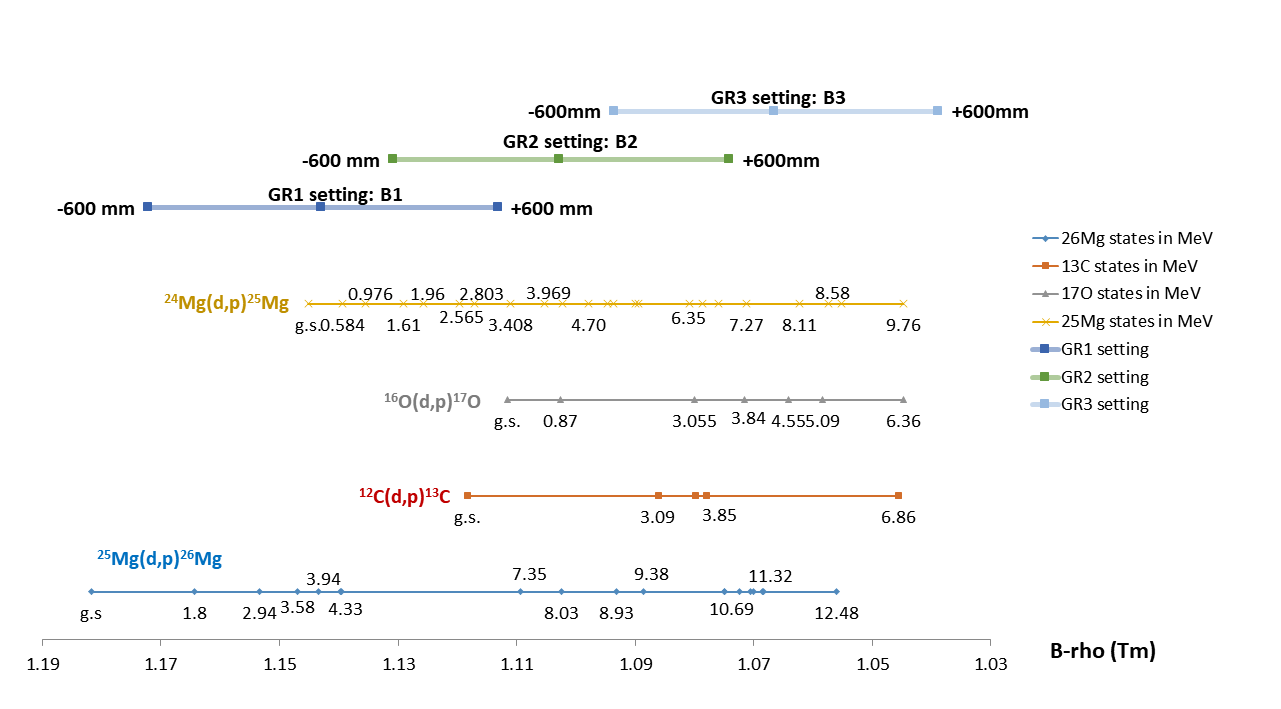
\includegraphics[scale=0.8]{graph/ch5/brho}}
    \caption{B-rho map for the measured three spectrometer settings.}
    \label{fig:brho}
    \end{figure}
\end{landscape}

\begin{figure}[tpb]
  \begin{center}
    \centerline{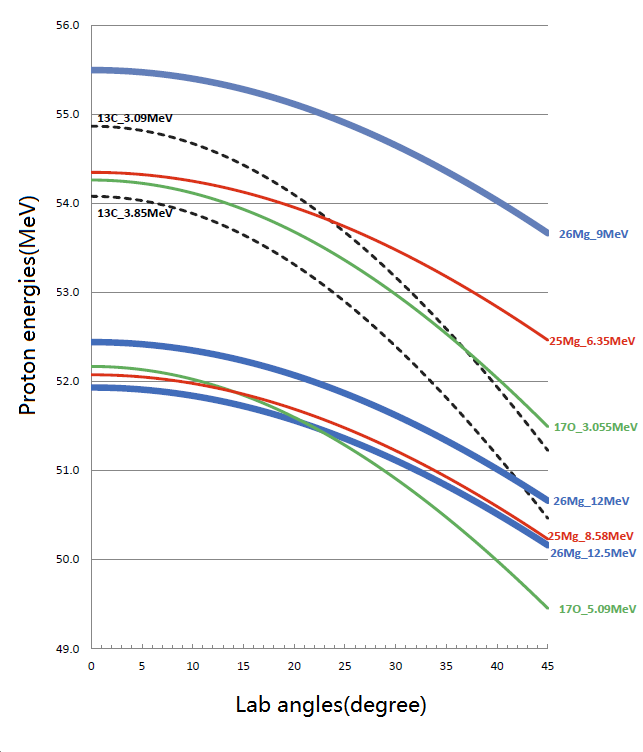
\includegraphics[scale=0.6]{graph/ch5/K}}
    \caption{Kinematic calculation of possible reaction products by proton energies versus  lab angles. Excited states of different targets could be identified by their different angular dependencies.}
    \label{fig:K}
  \end{center}
\end{figure}


\begin{figure}[tpb]
  \begin{center}
    \centerline{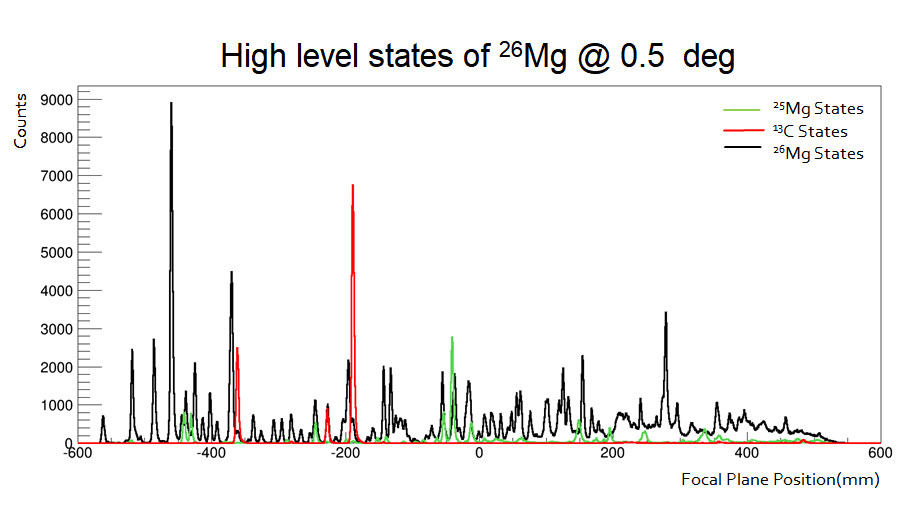
\includegraphics[scale=0.7]{graph/ch5/peaks}}
    \caption{Spectrum showing $^{12}$C(d,p)$^{13}$C, $^{24}$Mg(d,p)$^{25}$Mg and $^{25}$Mg(d,p)$^{26}$Mg for the third GR setting (B3). Energy range is from 8.5 MeV to 13 MeV.}
    \label{fig:peaks}
  \end{center}
\end{figure}

Peak normalization was performed in order to determine the contribution of each contamination peak in the $^{26}$Mg spectrum. This was done by first normalizing the spectrum with respect to the beam charges collected in each run. Then  the $^{26}$Mg spectrum was further improved by removing the identified contaminants. 



In this work all the contamination peaks had almost negligible contribution to the
$^{26}$Mg peaks.

\section{Peak Fitting}
To determine the centroid of each peak, the Right-skewed Gaussian function  was used to fit peaks as it gave lower reduced $\chi^2$ compared to a pure Gaussian shape. Right-skew rather than left-skew  was used because an electron energy shift occurs regularly toward the lower energies side, due to the incomplete charge collection in the detector. The formalism for a Right-skewed Gaussian function is defined as
\begin{equation}
    \label{eq:right_skew_gaus}
    \begin{aligned}
 f(x) & =  A \times \frac{\sqrt{\pi}}{2} \sigma \times RA \times \exp{\left[\left(\frac{\sigma}{2\times RS}\right)^2-\frac{x-x_0}{RS}\right]} \times erfc \left( \frac{\sigma}{RS} - \frac{x-x_0}{\sigma}\right) \\
      & + a x^2 + b x + c
    \end{aligned}
\end{equation}
where

$A$: Amplitude of Gaussian

$\sigma$: Gaussian width (Width = FWHM/1.66)

$x_0$: Position of the Gaussian centroid

$RA$: Right-skew amplitude relative to that of Gaussian

$RS$: Right-skew slope

$erfc$: Standard complementary error function

$a$, $b$, and $c$: Parameters of the second order polynomial background function.
Fig.~\ref{fig:fitting} shows an example of the total fit and the associated individual components obtained using Eq.~\ref{eq:right_skew_gaus}. %Table~\ref{tb:high} lists the energies of states of interest above the neutron threshold together with the the possible spin-parity values.
The Gaussian width $\sigma$ for $^{26}$Mg peaks populated by the $^{25}$Mg(d,p)$^{26}$Mg reaction was fixed for spectra at the same spectrometer angle settings.

\begin{figure}[tpb]
  \begin{center}
    \centerline{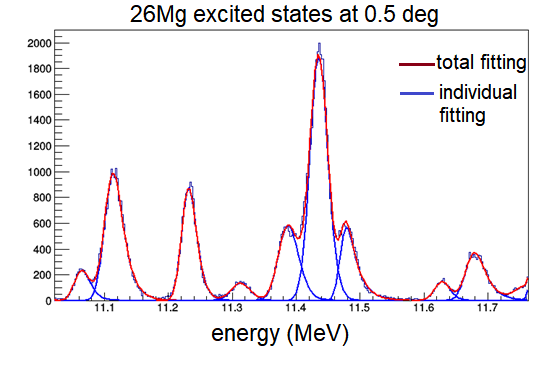
\includegraphics[scale=0.8]{graph/ch5/fitting}}
    \caption{Example of fitting results from Eq.~\ref{eq:right_skew_gaus}. Data from high-lying states of $^{26}$Mg at 0.5$^{\circ}$}
    \label{fig:fitting}
  \end{center}
\end{figure}

%x_error
The error of the peak position measurement consists of the systematic error given by  the peak fitting($\Delta x_{fit}$) and the statistical error ($\Delta x_{stat}$) due to the limited counting numbers defined by
\begin{equation}
    \label{eq:x_stat}
    \begin{aligned}
       \Delta x_{stat} = \frac{FWHM}{\sqrt{N}},
    \end{aligned}
\end{equation}
where $N$ is the integral of counts under each fitted peak. The total error of the peak position is calculated by the square root sum of the two components:
\begin{equation}
    \label{eq:x_error}
    \begin{aligned}
       \Delta x = \sqrt{\Delta x^2_{fit} + \Delta x^2_{stat}}.
    \end{aligned}
\end{equation}

\section{Energy Calibration}

The energy calibration was established using the $^{25}$Mg(d,p)$^{26}$Mg reaction at 0.5$^{\circ}$. The low-lying excited states of $^{26}$Mg are well-known\citep{Cujec1964} so their positions on the focal plane can be used to perform the absolute excitation energy calibration  as shown in Fig.\ref{fig:brho}.

As scattered particles travel through the Grand Raiden (GR) spectrometer, their bending radii in the magnetic dipole  field depend on the momentum following the equation:
\begin{equation}
    \label{eq:brho}
    \begin{aligned}
       B\rho = \frac{p}{q},
    \end{aligned}
\end{equation}
where $B$ is the magnetic field of the GR setting, $\rho$  the orbital radius, and $p$ and $q$  the momenta and the charge states of the scattered particle, respectively. $B\rho$ is  the magnetic rigidity of the detected particles and is associated with the focal plane position ($x_{fp}$). The excitation energy of the residual nuclei can be calculated by solving the two-body scattering kinematics Eq. \ref{eq:kinematic} once $B\rho$ and $q$ are known.
\begin{equation}
    \label{eq:kinematic}
    \begin{aligned}
 E_x = & \left(  { m^2_{in} + m^2_{tar} + m^2_{out} + 2E_{in}m_{tar}-2E_{out}m_{tar}}  \right. \\
       & \left.  { -2 E_{in}E_{out}+2p_{in}p_{out}\cos\theta_{lab} }        \right) ^{1/2} -m_{res} \\
    \end{aligned}
\end{equation}
where $m_{in}$, $m_{tar}$, $m_{out}$ and $m_{res}$ are the masses of the incident beam, target nuclei, outgoing particles and the residual nuclei, respectively. $E_x$, $E_{in}$ and $E_{out}$ are the energies of the excited states, incident  particles and outgoing particles, respectively. $p_{in}$, $p_{out}$ and $\theta_{lab}$ are the momenta of the incident and outgoing particles and the scattering angles in the lab frame. Since the energy losses of particles in the target need to be taken into account in the kinematic calculations, it is assumed that on average the $^{25}$Mg(d,p)$^{26}$Mg occurs at the center of the target. Therefore, the kinematic terms $E_{in}$, $E_{out}$, $p_{in}$ and $p_{out}$ were determined by the following equations:
\begin{equation}
    \label{eq:kinematic2}
    \begin{aligned}
        E_{in}  = m_{in} + T_{in} - E_{loss1} \\
        E_{out} = \sqrt{m_{out}^2 + p^2_{out}} + E_{loss2} \\
        p_{in}  = \sqrt{E_{out}^2-m_{in}^2}   \\
        p_{out} = \sqrt{E_{out}^2 - m_{out}^2}
     \end{aligned}
\end{equation}
where $E_{loss1}$ and $E_{loss2}$ refer to the energy loss of deuterons in the target prior to the reaction, and the protons after the reaction, respectively. This was calculated by the Stopping and Range of Ions in Matter (SRIM) program\citep{srim}. $T_{in}$ represents the kinematic energy of the incident beam. $p_{out}$ is the momentum of the scattered particles whose movements are described by Eq. \ref{eq:brho}. Therefore, once the magnetic rigidities of the detected particles in the focal plane are known, the excitation energies of the corresponding recoil nuclei can be calculated.

To determine the relationship between the measured $x_{fp}$ and $B\rho$, a function quadratic in $x_{fp}$ was used. In addition, as mentioned in the previous section,  three spectrometer  settings were used by changing the magnetic fields with sufficient overlap between the different spectra.

Finally, the calibration function is following the form:
\begin{equation}
    \label{eq:focal_plane_cali}
    \begin{aligned}
    B\rho /B\rho_0 = (ax_{fp}^2+bx_{fp}+c)/( 1.1597 \ T\cdot m)
    \end{aligned}
\end{equation}
where $x_{fp}$ is the corrected focal plane position after the software corrections. The quantity  1.1597 $T\cdot m$ is the magnetic rigidity of the first excited state of $^{26}$Mg.

The focal plane calibration obtained above is derived from the well-known low-lying states of $^{26}$Mg that were populated in the first spectrometer setting (B1). It could not be directly applied to the other two spectrometer  settings, for example, the third setting (B3) that corresponds to the region of our interest. However, since each setting was scaled to the next one, the initial focal plane calibration can also be scaled to the other focal plane settings by using the scaling factors obtained during the experiment:
\begin{equation}
    \label{eq:scaling}
    \begin{aligned}
    B\rho  =  \frac{B_2}{B_1}(ax_{}^2+bx_{}+c).
    \end{aligned}
\end{equation}
where $\dfrac{B_2}{B_1}$ represents the scaling factor between two different settings.



%%%
%b-rho : g.s. 1.1770
%b-rho : 1st  1.1597
\begin{figure}[tpb]
  \begin{center}
    \centerline{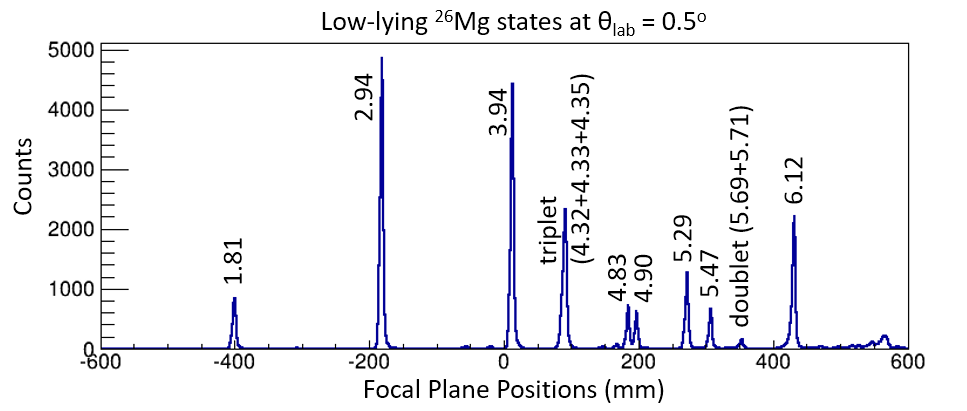
\includegraphics[scale=0.6]{graph/ch5/mg26_low}}
    \caption{Spectrum of low-lying $^{26}$Mg states populated by the $^{25}$Mg(d,p)$^{26}$Mg reaction at $\theta_{lab}$ = 0.5$^{\circ}$ under the first spectrometer setting. Level energies are taken from\citep{Cujec1964}}
    \label{fig:lowlying}
  \end{center}
\end{figure}

\begin{table}[tpb]
    \setlength{\capwidth}{0.7\textwidth}
    \begin{centering}
       \caption{WELL-KNOWN STATES USED IN THE ENERGY CALIBRATION}
       \label{tb:wellknown_states}
       \begin{tabular}{c c c}
       \toprule
       \toprule
          Well-known $^{26}$Mg States from NNDC~\citep{NNDC}  & Magnetic Rigidity & Focal Plane Position   \\
         (MeV) &(T $\cdot$ m)& (mm) \\
         \hline
         1.80874(4)  & 1.16429 & -400.691   \\
         2.93833(4)  & 1.15328 & -181.612   \\
         3.94157(4)  & 1.14342 & 12.396   \\
         4.83513(5)  & 1.13458 & 184.390   \\
         4.90144(7)  & 1.13392 & 197.105   \\
         5.29174(6)  & 1.11300 & 271.915   \\
         5.47605(7)  & 1.12819 & 307.048   \\
         6.12547(5)  & 1.12168 & 430.729   \\
         \hline
       \end{tabular}
     \end{centering}
\end{table}

\begin{figure}[tpb]
  \begin{center}
    \centerline{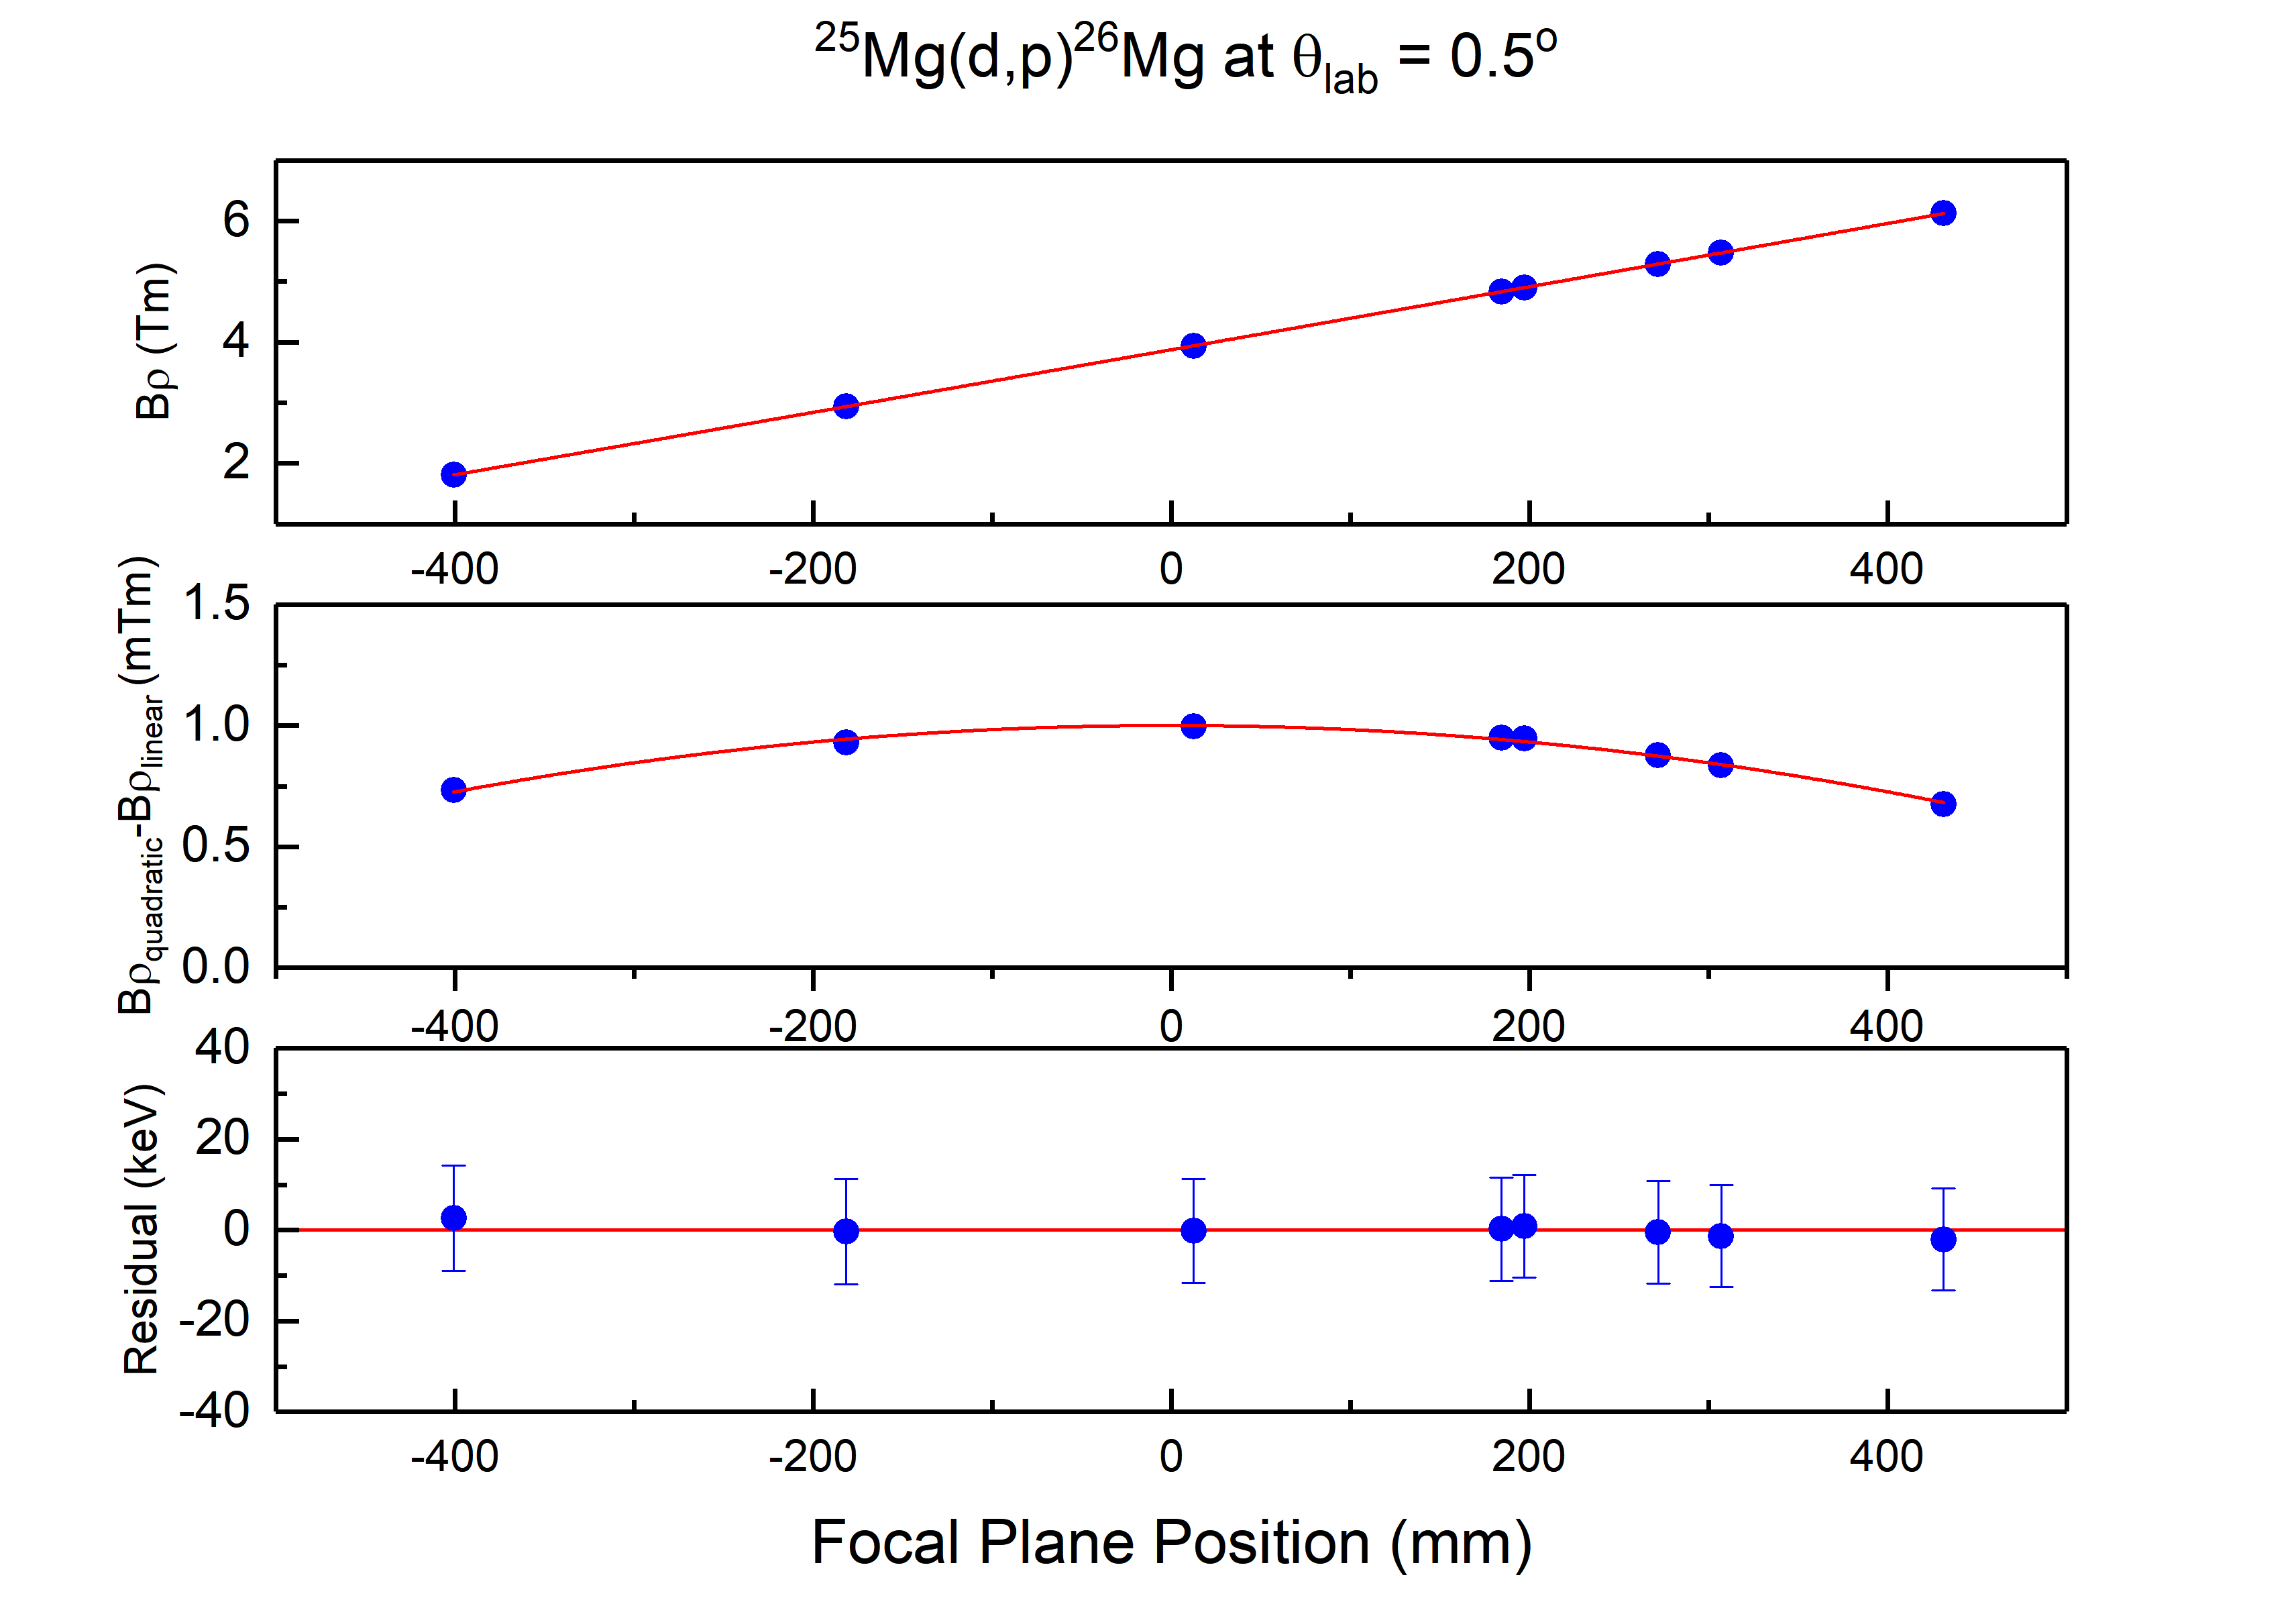
\includegraphics[scale=0.4]{graph/ch5/focalplane}}
    \caption{Focal plane calibration. Top panel: quadratic fitting . Middle panel: quadratic residual of the fit. Bottom panel: The deviation of the calibration from the actual data in terms of energy. }
    \label{fig:fp}
  \end{center}
\end{figure}

The determination of the fitting error of B$\rho$ in Eq. \ref{eq:focal_plane_cali} is  not straightforward since the calibration parameters  $a$, $b$ and $c$ are not  independent. Solving the covariance error matrix gives the systematic error $B\rho_{fit}$ by
\begin{equation}
    \label{eq:b-rho_fit}
    \begin{aligned}
    \delta B \rho^2_{fit} &=   (\frac{\partial B\rho}{\partial a})^2 (\delta a)^2 + (\frac{\partial B\rho}{\partial b})^2 (\delta b)^2 + (\frac{\partial B\rho}{\partial c})^2 (\delta c)^2 \\
                    & + \frac{\partial B\rho}{\partial a} \frac{\partial B\rho}{ \partial b} \delta a \delta b
                     + \frac{\partial B\rho}{\partial a} \frac{\partial B\rho}{ \partial c} \delta a \delta c
                     + \frac{\partial B\rho}{\partial b} \frac{\partial B\rho}{ \partial c} \delta b \delta c    \\
    \end{aligned}
\end{equation}
where $\delta a$, $\delta b$ and $\delta c$ are  covariant matrix terms.

The other type of error in the fitting is the error regarding the peak position:
\begin{equation}
    \label{eq:b-rho_pos}
    \begin{aligned}
    \delta B \rho_{c}^2 &=   (\frac{\partial B\rho}{\partial x})^2 (\Delta x)^2
    \end{aligned}
\end{equation}
where $\Delta x$ is obtained from Eq. ~\ref{eq:x_error}.

The final error of the magnetic rigidities can be expressed as
\begin{equation}
    \label{eq:b-rho_tot}
    \begin{aligned}
    \delta B \rho^2 &= B\rho_{c}^2 + B\rho_{fit}^2 \\
                    &=  (\frac{\partial B\rho}{\partial x})^2 (\Delta x)^2
                     + (\frac{\partial B\rho}{\partial a})^2 (\delta a)^2 + (\frac{\partial B\rho}{\partial b})^2 (\delta b)^2 + (\frac{\partial B\rho}{\partial c})^2 (\delta c)^2 \\
                    & + \frac{\partial B\rho}{\partial a} \frac{\partial B\rho}{ \partial b} \delta a \delta b
                     + \frac{\partial B\rho}{\partial a} \frac{\partial B\rho}{ \partial c} \delta a \delta c
                     + \frac{\partial B\rho}{\partial b} \frac{\partial B\rho}{ \partial c} \delta b \delta c    \\
    \end{aligned}
\end{equation}

The final schematic error of the excitation energy calculated from  Eq. ~\ref{eq:kinematic} was determined by the propagation of the errors from terms that were associated with $E$, including the error of particle energy loss in targets given by SRIM and the error associated with the atomic mass  ~\citep{mass_excess}.


The $^{26}$Mg energy levels in the region of interests populated by the (d,p) reaction are listed in Table~\ref{tb:6Lid}, Table~\ref{tb:aa}, Table~\ref{tb:ddpp}, Table~\ref{tb:dp} and Table~\ref{tb:other}.

\section{Cross Section Calculation}

The differential cross section is defined by
\begin{equation}
    \label{eq:cross_section}
    \begin{aligned}
    \frac{d\sigma}{d\Omega} = \frac{Y}{N_B l N_0 \eta \Delta \Omega}  cm^2/sr
    \end{aligned}
\end{equation}
Where $Y$ is the reaction yields in the accepted solid angle $\Delta \Omega$ (in msr) while $\Delta \Omega$ was calculated from the $\theta_{tgt}$ and $\phi_{tgt}$ plot  and was determined to be  2.79 msr in this experiment.  $\eta$ is the efficiency of the total detection system (85\% in the experiment) as described in the previous chapter.  $N_0$ is the number of target nuclei per cm$^2$ determined from the target thickness $\Delta x$, and $N_B$ is  the total number of incident particles which depends on the integrated current of the incident  beam $Q$, the atomic charge $Z$ and the electron charge $e$. The live time ratio $l$ of the detection system varied from 93\% to 96\%.
%$N_B$ is the number of incident beam particles.

The cross-section measurement near 0$^{\circ}$  required a different Faraday cup compared to those at higher angles. As shown in Fig. 3.8 ( Chapter 3), in the  0$^{\circ}$ measurement the Faraday cup was placed inside the first dipole  D1 (D1FC).  For the angle at 5$^{\circ}$  the Faraday cup Q1FC downstream of the quadrupole  Q1 was used. For larger angles the Faraday cup in the scattering chamber (SCFC) was employed. Measurements at small angles by D1FC and Q1FC need to be normalized to SCFC since SCFC has an effective electron suppression
system. Faraday cup normalization between the different modes was achieved by monitoring the count rate on the D1FC and SCFC for several runs.







\section{Analysis of Energy Levels}

In this measurement of $^{25}$Mg(d,p)$^{26}$Mg, 102 energy levels were populated above the first excited states up to 12.311 MeV.
Considerable effort has been made in the past by various methods to probe the $^{26}$Mg resonances in the astrophysical region of interest. The reaction mechanism of each reaction  focuses on different aspects in terms of the input parameters into the  reaction rate calculation.
The (d,p) reactions used in this work populate more or less every state but the strength depends on the strength of the single particle component in the wave function.
The excited states of $^{26}$Mg in the present work will be compared with  the states populated by several different reactions, including
the reaction $^{22}$Ne($^6$Li,d)$^{26}$Mg by Ugalde $et\ al.$\citep{Ugalde2007}, Giesen $et\ al.$\citep{GIESEN199395} and Talwar $et\ al.$\citep{Rashi2016},
the reaction $^{26}$Mg($\alpha$,$\alpha'$)$^{26}$Mg by Talwar $et\ al.$\citep{Rashi2016} and Adsley $et\ al.$\citep{26mgaa2017},
the inelastic scattering $^{26}$Mg(p,p$'$)$^{26}$Mg and  $^{26}$Mg(d,d$'$)$^{26}$Mg by Adsley $et\ al.$\citep{26mgdd2018} and Moss $et\ al.$ \citep{Moss1967},
the reactions $^{25}$Mg(d,p)$^{26}$Mg by Cujec $et\ al.$\citep{Cujec1964}, Hinds $et\ al.$\citep{Hinds1965}\citep{Hinds1961} and Arciszewski $et\ al.$\citep{Arciszewski1984}, along with data from the n-ToF $^{25}$Mg(n,$\gamma$) measurement by Massimi $et\ al.$\citep{Massimi}\citep{MASSIMI2017},
and the last comparison will be among reactions $^{23}$Na($\alpha$,p$\gamma$)$^{26}$Mg and $^{12}$C($^{18}$O,$\alpha$)$^{26}$Mg by Glatz $et\ al.$\citep{Glatz1986} and Gustafson $et\ al.$ \citep{Gustafson1976}, respectively.
%%%%%%%%%%%%





\subsection{Comparison with the  reaction $^{22}$Ne($^6$Li,d)$^{26}$Mg}

Studies of the $\alpha$-transfer on $^{22}$Ne have been performed \citep{GIESEN199395}\citep{Ugalde2007}\citep{Rashi2016} and several states with strong $\alpha$ structure have been observed and is listed in Table~\ref{tb:6Lid}. These measurements also provided critical information on the $\alpha$-widths for states above the $\alpha$-threshold which contribute to reaction rate calculation for the $^{22}$Ne + $\alpha$ system. Since no  ($\alpha$,n) resonance strength was determined in the $\alpha$-channel in this work,  the data from $\alpha$-transfer data is needed.  Giesen $et\ al.$\citep{GIESEN199395} reported two natural parity resonances (E$_x=$10.694(20) MeV and E$_x=$10.949(25) MeV) between the  $\alpha$- and $n$- thresholds with the resolution of 120 keV.  Ugalde $et\ al.$\citep{Ugalde2007} subsequently improved the resolution to 63 keV in the region of interest.   Talwar $et\ al.$\citep{Rashi2016} observed and used additional resonances to the reaction rate calculation with the resolution of 100 keV.
However, due to the fact that the $\alpha$-transfer reaction only populates natural parity states and favors states with a strong $\alpha$ structure, it  gives a lower number of states comparing to the (d,p) reaction. Other than that, the energy levels in the present work are mostly consistent with  the previous ($^6$Li,d) measurements, despite one weakly populated state E$_x=$11.644(20) MeV in Giesen $et\ al.$'s work is not observed in the present measurements.


%%%%%%%%%%%%%%%%%6Lid

\begin{center}
%\setlength{\LTleft}{0pt} \setlength{\LTright}{0pt}
%\setlength{\tabcolsep}{7mm}
%%   \begin{ThreePartTable}
    \begin{longtable}{cc c cc cc}
    %\setlength{\LTleft}{0pt} \setlength{\LTright}{0pt}
    \caption{COMPARISONS WITH STATES of $^{26}$MG POPULATED BY THE ($^6$LI,D) REACTION \label{tb:6Lid}\/}\\
    \toprule
    \hline
    \multicolumn{2}{c}{This Work}          & Ugalde $et\ al.$\citep{Ugalde2007}    & \multicolumn{2}{c}{Giesen $et\ al.$\citep{GIESEN199395}}  & \multicolumn{2}{c}{Talwar $et\ al.$\citep{Rashi2016}} \\
    \multicolumn{2}{c}{($d,p$)}            &              ($^6Li,d$)               & \multicolumn{2}{c}{($^6 Li,d$)}      & \multicolumn{2}{c}{($^6 Li,d$)}     \\
      $E_x$(MeV)  &  $l_n$                 & $E_x$(MeV)                            &  $E_x$(MeV)   & $J^{\pi}$             & $E_x$(MeV)   & $J^{\pi}$             \\
    \midrule
    \endfirsthead % Everything above goes at the top of the 1st page only
% As with the first header, we don't want obscene amounts of space for
% subsequent headings either, and eliminate an em of whitespace.
  \caption[]{{\em Continued}}\\
    \midrule
    \hline
    \multicolumn{2}{c}{This Work}          & Ugalde $et\ al.$\citep{Ugalde2007}    & \multicolumn{2}{c}{Giesen $et\ al.$\citep{GIESEN199395}}  & \multicolumn{2}{c}{Talwar $et\ al.$\citep{Rashi2016}} \\
    \multicolumn{2}{c}{($d,p$)}            &              ($^6Li,d$)               & \multicolumn{2}{c}{($^6 Li,d$)}      & \multicolumn{2}{c}{($^6 Li,d$)}     \\
      $E_x$(MeV)  &  $l_n$                 & $E_x$(MeV)                            &  $E_x$(MeV)   & $J^{\pi}$             & $E_x$(MeV)   & $J^{\pi}$             \\
    \midrule
    \endhead
    \endfoot % The above section goes at the bottom of continuation pages
  \bottomrule

\endlastfoot

  7.347 (12)    &       &                   &                   &                   &    7.365(13)      &  2$^+$            \\
  7.540 (11)    &       &                   &                   &                   &                   &                   \\
  7.677 (11)    &       &                   &                   &                   &    7.671(16)      &                   \\
  7.712 (12)    &       &                   &                   &                   &                   &                   \\
  7.733 (11)    &       &                   &                   &                   &                   &                   \\
  7.809 (11)    &       &                   &                   &                   &    7.821(22)      &  3$^-$            \\
  7.942 (10)    &       &                   &                   &                   &                   &                   \\
  7.996 (11)    &       &                   &                   &                   &                   &                   \\
  8.042 (11)    &       &                   &                   &                   &    8.040(13)      &   2$^+$           \\
  8.179 (12)    &       &                   &                   &                   &    8.214(14)      &   6$^+$           \\
  8.243 (12)    &       &                   &                   &                   &                   &                   \\
  8.393 (11)    &       &                   &                   &                   &                   &                   \\
  8.454 (10)    &       &                   &                   &                   &                   &                   \\
  8.497 (11)    &       &                   &                   &                   &                   &                   \\
  8.527 (11)    &       &                   &                   &                   &                   &                   \\
  8.621 (11)    &       &                   &                   &                   &    8.625(15)      &   5$^-$           \\
  8.706 (11)    &       &                   &                   &                   &                   &                   \\
  8.865 (11)    &       &                   &                   &                   &                   &                   \\
  8.904 (10)    &       &                   &                   &                   &                   &                   \\
 8.931 (11)     &       &                   &                   &                   &    8.931(13)      &   1$^-$,2$^+$     \\
  8.960 (11)    &       &                   &                   &                   &                   &                   \\
   9.052 (11)   &       &                   &                   &                   &                   &                   \\
  9.167 (11)    &       &                   &                   &                   &                   &                   \\
  9.238 (12)    &       &                   &                   &                   &                   &                   \\
  9.263 (11)    &       &                   &                   &                   &                   &                   \\
   9.322(11)    &       &     9.32(6)       &                   &                   &                   &                   \\
  9.382 (11)    &       &                   &                   &                   &    9.383(16)      &  0$^+$,1$^-$      \\
  9.430 (11)    &       &                   &     9.404(20)     & (4$^+$), 6$^+$    &                   &                   \\
  9.476 (11)    &       &                   &                   &                   &                   &                   \\
   9.578(11)    &       &     9.57(4)       &    9.586(20)      &   4$^+$           &   9.595(32)       &  1$^-$,2$^+$      \\
   9.613(11)    &       &                   &                   &                   &                   &                   \\
  9.683 (10)    &       &                   &                   &                   &                   &                   \\
  9.716 (11)    &       &                   &                   &                   &                   &                   \\
  9.770 (11)    &       &                   &                   &                   &                   &                   \\
  9.856 (11)    &       &                   &                   &                   &                   &                   \\
  9.985 (11)    &       &                   &     9.985(20)     &                   &    9.987(18)      & 1$^-$,2$^+$       \\
  9.991 (11)    &       &                   &                   &                   &                   &                   \\
  10.040(10)    &       &                   &                   &                   &                   &                   \\
  10.100(10)    &       &                   &                   &                   &                   &                   \\
  10.137(11)    &       &                   &                   &                   &                   &                   \\
  10.269(11)    &       &                   &                   &                   &                   &                   \\
  10.320(11)    &       &                   &                   &                   &                   &                   \\
  10.355(12)    &       &                   &     10.335(20)    &   (7$^-$)         &   10.357(14)      & 2$^+$             \\
  10.385(12)    &       &                   &                   &                   &                   &                   \\
  10.487(12)    &       &                   &                   &                   &                   &                   \\
  10.522(11)    &       &                   &                   &                   &                   &                   \\
  10.568(11)    &       &                   &    10.568(25)     &                   &                   &                   \\
  10.595(11)    &       &                   &                   &                   &                   &                   \\
 10.641(11)     &       &                   &                   &                   &                   &                   \\
 10.676(11)     &       &                   &                   &                   &                   &                   \\
 10.708(10)     &   1   &                   &     10.694(20)    &4$^+$,7$^-$,8$^+$  &    10.714(20)     & 1$^-$,2$^+$,4$^+$ \\
 10.735(11)     &   2   &                   &                   &                   &                   &                   \\
 10.808(10)     &   2   &     10.808(20)    &     10.949(25)    &(2$^+$,4$^+$)3$^-$ &   10.977(15)      &1$^-$,2$^+$,4$^+$  \\
 10.875(11)     &   3   &                   &                   &                   &                   &                   \\
 10.915(10)     &   2   &                   &                   &                   &                   &                   \\
10.988(11)      &   3   &     10.953(25)    &                   &                   &                   &                   \\
 11.069(10)     &   2   &                   &                   &                   &                   &                   \\
  11.112(11)    &   3   &                   &                   &                   &                   &                   \\
 11.165(10)     &   1   &                   &                   &                   &   11.169(17)      &       1$^-$       \\
 11.232(10)     &   2   &                   &                   &                   &                   &                   \\
 11.267(10)     &   2   &                   &                   &                   &                   &                   \\
 11.317(11)     &   3   &                   &     11.310(20)    &  (1$^-$),2$^+$    &   11.317(18)      &       1$^-$       \\
 11.374(12)     &   3   &                   &                   &                   &                   &                   \\
 11.425(12)     &   2   &                   &                   &                   &                   &                   \\
 11.447(11)     &   3   &                   &     11.453(25)    &(1$^-$,2$^+$),3$^-$&                   &                   \\
 11.482(10)     &   1   &                   &                   &                   &                   &                   \\
 11.509(10)     &   3   &                   &                   &                   &                   &                   \\
  11.573(11)    &   3   &                   &                   &                   &                   &                   \\
  11.613(11)    &   2   &                   &                   &                   &                   &                   \\
                &       &                   &     11.644(20)    &                   &                   &                   \\
   11.690(10)   &   1   &                   &                   &                   &                   &                   \\
   11.767(11)   &   3   &                   &                   &                   &                   &                   \\
   11.790(11)   &   2   &                   &                   &                   &                   &                   \\
   11.828(10)   &   3   &                   &     11.831(20)    &(1$^-$,2$^+$,3$^-$)&                   &                   \\
     11.874(11) &   2   &                   &                   &                   &                   &                   \\
    11.927(11)  &   3   &                   &                   &                   &                   &                   \\
    11.981(11)  &   2   &                   &                   &                   &                   &                   \\
     12.032(11) &   1   &                   &                   &                   &                   &                   \\
     12.059(12) &   3   &                   &                   &                   &                   &                   \\
    12.311(11)  &   1   &                   &                   &                   &                   &                   \\


    \end{longtable}
\end{center}




\subsection{Comparison with the reaction $^{26}$Mg($\alpha$,$\alpha'$)$^{26}$Mg}

Talwar $et\ al.$\citep{Rashi2016} and Adsley $et\ al.$\citep{26mgaa2017} have made the similar measurements using the $^{26}$Mg($\alpha$,$\alpha'$)$^{26}$Mg reaction. This reaction preferentially populates natural parity states with low-spins.  In addition to the the fixed peak positions with known excitation energies, an additional resonance at E$_x$=10.89(1) MeV was observed in Adsley $et\ al.$'s work at small angle measurements (4${^\circ}<\theta_{lab}< $5$^{\circ}$ and 5${^\circ}<\theta_{lab}< $6$^{\circ}$). Owing to the poor resolution in Talwar $et\ al.$'s measurements (65 keV compared to 53 keV from Asdley $et\ al.$'s small angle data), this weakly populated state was only seen in Asdley $et\ al.$'s work. This state might correspond to the 10.881 MeV or 10.893 MeV observed by Moss\citep{Moss1967} or 10.875(11) or 10.915(10) MeV observed in this work.
Since only $l=0$ and $l=1$ transitions can be made in the ($\alpha$,$\alpha'$) reaction, while the transferred neutrons in the present work  brought higher momenta,  there are differences in the spin-parity assignments of the two experiment methods (See Table~\ref{tb:aa}).

\begin{center}
%\setlength{\LTleft}{0pt} \setlength{\LTright}{0pt}
%\setlength{\tabcolsep}{7mm}
    \begin{longtable}{cc cc cc}
    %\setlength{\LTleft}{0pt} \setlength{\LTright}{0pt}
    \caption{COMPARISONS WITH STATES of $^{26}$MG POPULATED BY THE ($\alpha,\alpha'$) REACTION \label{tb:aa}\/}\\
    \toprule
    \hline
    \multicolumn{2}{c}{This Work}& \multicolumn{2}{c}{Talwar $et\ al.$\citep{Rashi2016}}  & \multicolumn{2}{c}{Adsley $et\ al.$\citep{26mgaa2017}} \\
    \multicolumn{2}{c}{($d,p$)}  & \multicolumn{2}{c}{($\alpha,\alpha'$)} & \multicolumn{2}{c}{($\alpha,\alpha'$)}\\
      $E_x$(MeV) &  $l_n$        &  $E_x$(MeV)   & $J^{\pi}$             & $E_x$(MeV)    & $J^{\pi}$            \\
    \midrule
    \endfirsthead % Everything above goes at the top of the 1st page only
% As with the first header, we don't want obscene amounts of space for
% subsequent headings either, and eliminate an em of whitespace.
  \caption[]{{\em Continued}}\\
    \midrule
    \hline
    \multicolumn{2}{c}{This Work}& \multicolumn{2}{c}{Talwar $et\ al.$\citep{Rashi2016}}  & \multicolumn{2}{c}{Adsley $et\ al.$\citep{26mgaa2017}} \\
    \multicolumn{2}{c}{($d,p$)}  & \multicolumn{2}{c}{($\alpha,\alpha'$)} & \multicolumn{2}{c}{($\alpha,\alpha'$)}\\
      $E_x$(MeV) &  $l_n$        &  $E_x$(MeV)   & $J^{\pi}$             & $E_x$(MeV)    & $J^{\pi}$            \\

    \midrule
    \endhead
    \endfoot % The above section goes at the bottom of continuation pages
  \bottomrule

\endlastfoot
  7.677 (11)      &          &  7.685(8)        &                     &             &                 \\
  7.712 (12)      &          &                  &                     &             &                 \\
  7.733 (11)      &          &                  &                     &             &                 \\
  7.809 (11)      &          &  7.826(6)        &                     &             &                 \\
  7.942 (10)      &          &                  &                     &             &                 \\
  7.996 (11)      &          &                  &                     &             &                 \\
  8.042 (11)      &          &  8.036(7)        &                     &             &                 \\
  8.179 (12)      &          &  8.193(15)       &                     &             &                 \\
  8.243 (12)      &          &                  &                     &             &                 \\
  8.393 (11)      &          &                  &                     &             &                 \\
  8.454 (10)      &          &                  &                     &             &                 \\
  8.497 (11)      &          &  8.497(8)        &                     &             &                 \\
  8.527 (11)      &          &                  &                     &             &                 \\
  8.621 (11)      &          &  8.626(7)        &                     &             &                 \\
  8.706 (11)      &          &  8.703(6)        &                     &             &                 \\
   8.865(11)      &          &  8.866(9)        &                     &             &                 \\
  8.904 (10)      &          &                  &                     &             &                 \\
  8.931(11)       &          &  8.937(6)        &                     &             &                 \\
  8.960 (11)      &          &                  &                     &             &                 \\
   9.052(11)      &          &                  &                     &             &                 \\
  9.167 (11)      &          &                  &                     &             &                 \\
  9.238 (12)      &          &                  &                     &             &                 \\
  9.263 (11)      &          &  9.276(10)       &                     &             &                 \\
   9.322(11)      &          &                  &                     &             &                 \\
  9.382 (11)      &          &  9.383(16)       &                     &             &                 \\
  9.430 (11)      &          &                  &                     &             &                 \\
  9.476 (11)      &          &                  &                     &             &                 \\
   9.578(11)      &          &                  &                     &             &                 \\
   9.613(11)      &          &  9.603(9)        &                     &             &                 \\
  9.683 (10)      &          &                  &                     &             &                 \\
  9.716 (11)      &          &  9.718(7)        &                     &             &                 \\
  9.770 (11)      &          &                  &                     &             &                 \\
  9.856 (11)      &          &  9.863(6)        &                     &             &                 \\
  9.985 (11)      &          &                  &                     &             &                 \\
  9.991 (11)      &          &  9.992(9)        &                     &             &                 \\
  10.040(10)      &          &                  &                     &             &                 \\
                  &          &  10.067(7)       &                     &             &                 \\
  10.100(10)      &          &                  &                     &             &                 \\
  10.137(11)      &          &  10.136(8)       &                     &             &                 \\
  10.269(11)      &          &  10.273(10)      &                     &             &                 \\
  10.320(11)      &          &                  &                     &             &                 \\
  10.355(12)      &          &  10.350(7)       &                     &             &                 \\
  10.385(12)      &          &                  &                     &             &                 \\
  10.487(12)      &          &  10.495(9)       & 1$^-$               & 10.495(9)   &  1$^-$          \\
  10.522(11)      &          &                  &                     &             &                 \\
10.568(11)        &          &  10.575(10)      & 1$^-$,2$^+$         & 10.5733(8)  &  1$^-$          \\
  10.595(11)      &          &                  &                     &             &  1$^-$          \\
     10.641(11)   &          &                  &                     &             &                 \\
     10.676(11)   &          &                  &                     &             &                 \\
     10.708(10)   & 1        &  10.717(9)       & 1$^-$,2$^+$         & 10.717(9)   &  2$^+$          \\
     10.735(11)   & 2        &                  &                     &             &                 \\
     10.808(10)   & 2        &                  &                     & 10.8057(7)  &  1$^-$          \\
                  &          &  10.822(10)      &   1$^-$             & 10.824(3)   &  0$^+$          \\
     10.875(11)   & 3        &                  &                     &             &                 \\
      10.915(10)  & 2        &                  &                     & 10.89(1)    &  $>$1           \\
                  &          &  10.951(21)      &  1$^-$,2$^+$        & 10.9491(8)  &  1$^-$          \\
   10.988(11)     & 3        &                  &                     &             &                 \\
    11.069(10)    & 2        &  11.085(8)       &  2$^+$,3$^-$        & 11.085(8)   &  2$^+$,3$^- $   \\
     11.112(11)   & 3        &                  &                     &             &                 \\
    11.165(10)    & 1        &  11.167(9)       &  1$^-$,2$^+$        & 11.167(8)   &  (2$^+$)        \\
    11.232(10)    & 2        &                  &                     &             &                 \\
    11.267(10)    & 2        &                  &                     &             &                 \\
    11.317(11)    & 3        &  11.301(9)       &  1$^-$,2$^+$,3$^-$  & 11.301(9)   &  $>$1           \\
                  &          &                  &                     & 11.3347(4)  &  $>$1           \\
                  &          &  11.359(8)       &  1$^-$,2$^+$        &             &                 \\
    11.374(12)    & 3        &                  &                     &             &                 \\
    11.425(12)    & 2        &                  &                     &             &                 \\
    11.447(11)    & 3        &  11.445(9)       &  1$^-$,3$^-$        & 11.441(2)   &  1$^-$,3$^-$    \\
    11.482(10)    & 1        &                  &                     &             &                 \\
    11.509(10)    & 3        &  11.509(11)      &  0$^+$,1$^-$        & 11.5001(4)  &  1$^-$          \\
                  &          &                  &                     & (11.526)    &  (1$^-$)        \\
     11.573(11)   & 3        &                  &                     &             &                 \\
     11.613(11)   & 2        &                  &                     &             &                 \\
                  &          &  11.648(7)       & 1$^-$,2$^+$         &             &                 \\
   11.690(10)     & 1        &                  &                     &             &                 \\
                  &          &  11.731(9)       & 1$^-$,2$^+$         &             &                 \\
   11.767(11)     & 3        &                  &                     &             &                 \\
   11.790(11)     & 2        &                  &                     &             &                 \\
   11.828(10)     & 3        &  11.824(9)       & 0$^+$,1$^-$         &             &                 \\
     11.874(11)   & 2        &                  &                     &             &                 \\
                  &          &  11.900(9)       & 1$^-$,2$^+$         &             &                 \\
    11.927(11)    & 3        &                  &                     &             &                 \\
    11.981(11)    & 2        &                  &                     &             &                 \\
     12.032(11)   & 1        &                  &                     &             &                 \\
     12.059(12)   & 3        &  12.064(8)       & 0$^+$,1$^-$,2$^+$   &             &                 \\
    12.311(11)    & 1        &                  &                     &             &                 \\

    \end{longtable}
\end{center}



\subsection{Comparison with the reactions $^{26}$Mg(p,p$'$)$^{26}$Mg and  $^{26}$Mg(d,d$'$)$^{26}$Mg}
The proton  inelastic scattering reaction can populate almost everything of $^{26}$Mg nucleus with no preferences on spins and parities. Adsley $et\ al.$\citep{26mgdd2018} and Moss $et\ al.$ \citep{Moss1967} have performed the reaction $^{26}$Mg(p,p$'$)$^{26}$Mg and probed the states of $^{26}$Mg above the $\alpha$- and neutron-threshold (See Table~\ref{tb:ddpp}).
Besides the states that were populated in both measurements, Adsley $et\ al.$ observed more states than  Moss $et\ al.$' work due to the achievement of a better resolution (6 keV compared to 6 - 12 keV).
Other than the $(p,p')$ reaction, the deuteron inelastic scattering reaction has been performed in  \citep{26mgdd2018} in order to obtain an additional verification of levels of $^{26}$Mg, as well as to evaluate the contribution to the $^{22}$Ne + $\alpha$ reaction  since the $(d,d')$ reaction is selective to isoscalar transitions. The possible new states observed in \citep{26mgdd2018} but not shown in  \citep{Moss1967} were E$_x=$ 10.943(2) MeV, 11.074(1) MeV, 11.102(1) MeV, 11.113(1) MeV, 11.119(1) MeV, 11.209(1) MeV, 11.266(1) MeV, 11.414(1) MeV, 11.426(1) MeV and 11.481(1) MeV. Among them E$_x=$ 10.943(2) MeV was seen only in the  $(d,d')$ reaction and E$_x=$ 11.113(1) MeV was not seen in the  $(d,d')$ reaction but seen in both $(p,p')$ reaction and this work.  E$_x=$ 11.074(1) might be  associated with E$_x=$ 11.069(10) MeV observed in this (d,p) reaction, while E$_x=$ 11.119(1) was the possible new state measured only in \citep{26mgdd2018}.  E$_x=$ 11.209(1) MeV, 11.216(1) MeV, 11.266(1) MeV, 11.414(1) MeV, 11.481(1) MeV and 11.481(1) MeV were only observed at one angle in  Adsley $et\ al.$'s $(p,p')$ measurements. However E$_x=$ 11.266(1) MeV,  11.414(1) MeV and 11.481(1) MeV can find the corresponding states in this work at all angle measurements, only E$_x=$ 11.209(1) MeV, 11.216(1) MeV and 11.414(1) MeV are not shown up in this (d,p) reaction, which can be explained by the possible $^{24}$Mg contaminants as stated in \citep{26mgdd2018}. Finally, although the states populated by the proton inelastic scattering reaction in \citep{26mgdd2018} and \citep{Moss1967}  were necessarily populated the same states as the $\alpha$ inelastic scattering discussed in the last subsection, the energy levels observed in  \cite{Rashi2016} and \cite{26mgaa2017} were all  consistent with the $(p,p')$ data and the additional resonance $E_x=$ 10.89(1) MeV in \cite{26mgaa2017} might be observed as 10.882(1) MeV and 10.881(3) MeV in \citep{26mgdd2018} and \citep{Moss1967}, respectively.



\begin{center}
%\setlength{\LTleft}{0pt} \setlength{\LTright}{0pt}
%\setlength{\tabcolsep}{7mm}
    \begin{longtable}{cc cc c}
    %\setlength{\LTleft}{0pt} \setlength{\LTright}{0pt}
    \caption{COMPARISONS WITH STATES of $^{26}$MG POPULATED BY THE (D,D\') and (P,P\') REACTIONS \label{tb:ddpp}\/}\\
    \toprule
    \hline
    \multicolumn{2}{c}{This Work} & \multicolumn{2}{c}{Adsley $et\ al.$\citep{26mgdd2018}}        &  Moss $et\ al.$ \citep{Moss1967}        \\
     \multicolumn{2}{c}{($d,p$)}  & \multicolumn{2}{c}{($p,p'$) and ($d,d'$)}                     & $(p,p')$                                \\
       $E_x$(MeV) &  $l_n$        &  $E_x$(MeV)   & $J^{\pi}$                                     & $E_x$(MeV)                              \\
    \midrule
    \endfirsthead % Everything above goes at the top of the 1st page only
% As with the first header, we don't want obscene amounts of space for
% subsequent headings either, and eliminate an em of whitespace.
  \caption[]{{\em Continued}}\\
    \midrule
    \hline
    \multicolumn{2}{c}{This Work} & \multicolumn{2}{c}{Adsley $et\ al.$\citep{26mgdd2018}}        &  Moss $et\ al.$ \citep{Moss1967}        \\
     \multicolumn{2}{c}{($d,p$)}  & \multicolumn{2}{c}{($p,p'$) and ($d,d'$)}                     & $(p,p')$                                \\
       $E_x$(MeV) &  $l_n$        &  $E_x$(MeV)   & $J^{\pi}$                                     & $E_x$(MeV)                              \\

    \midrule
    \endhead
    \endfoot % The above section goes at the bottom of continuation pages
  \bottomrule

\endlastfoot

     10.641(11)        &          & 10.650(1)   &            1$^+$              &    10.644(3)  \\
     10.676(11)        &          & 10.684(2)   &                               &    10.678(3)  \\
                       &          & 10.693(1)   &            4$^+$              &    10.689(3)  \\
     10.708(10)        & 1        & 10.706(1)   &                               &    10.702(3)  \\
                       &          & 10.719(2)   &            2$^+$              &    10.715(3)  \\
     10.735(11)        & 2        & 10.730(2)   &                               &    10.726(3)  \\
                       &          & 10.746(3)   &                               &    10.744(3)  \\
                       &          & 10.771(1)   &                               &    10.769(3)  \\
     10.808(10)        & 2        & 10.806(1)   &            1$^-$              &               \\
                       &          & 10.818(1)   &            1$^+$              &               \\
                       &          & 10.826(1)   &            0$^+$              &    10.824(3)  \\
     10.875(11)        & 3        & 10.882(1)   &                               &    10.881(3)  \\
                       &          & 10.893(1)   &                               &    10.893(3)  \\
     10.915(10)        & 2        & 10.915(1)   &                               &    10.915(3)  \\
                       &          & 10.928(1)   &                               &    10.927(3)  \\
                       &          & 10.943(2)   &                               &               \\
                       &          & 10.950(1)   &            1$^-$              &    10.950(3)  \\
                       &          & 10.978(1)   &                               &    10.978(3)  \\
   10.988(11)          & 3        & 10.998(1)   &                               &    10.998(3)  \\
                       &          & 11.017(1)   &                               &    11.017(3)  \\
                       &          & 11.047(1)   &                               &    11.048(3)  \\
    11.069(10)         & 2        & 11.074(1)   &                               &               \\
                       &          & 11.084(1)   &                               &    11.084(3)  \\
                       &          & 11.102(1)   &                               &               \\
     11.112(11)        & 3        & 11.113(1)   &            2$^+$              &               \\
                       &          & 11.119(1)   &                               &               \\
                       &          & 11.155(1)   &            1$^+$              &    11.156(3)  \\
    11.165(10)         & 1        & 11.165(1)   &            2$^+$ ,  3$^-$     &               \\
                       &          & 11.172(1)   &                               &    11.171(3)  \\
                       &          & 11.184(1)   &            (1$^-$)            &               \\
                       &          & 11.191(1)   &            3$^+$              &               \\
                       &          & 11.209(1)   &                               &               \\
                       &          & 11.216(1)   &                               &               \\
    11.232(10)         & 2        & 11.243(3)   &                               &               \\
                       &          & 11.245(1)   &            2$^-$              &               \\
    11.267(10)         & 2        & 11.266(1)   &                               &               \\
    11.317(11)         & 3        & 11.321(1)   &                               &               \\
                       &          & 11.329(1)   &           (1$^+$)             &               \\
                       &          & 11.345(1)   &                               &               \\
                       &          & 11.357(1)   &                               &               \\
    11.374(12)         & 3        &             &                               &               \\
                       &          & 11.395(1)   &                               &               \\
                       &          & 11.414(1)   &                               &               \\
    11.425(12)         & 2        & 11.426(1)   &                               &               \\
    11.447(11)         & 3        & 11.444(1)   & (4$^+$)$\rightarrow$J$\leq$3  &               \\
                       &          & 11.46(1)    &        1$^+$                  &               \\
                       &          & 11.467(1)   & (5$^-$)$\rightarrow$J$\leq$3  &               \\
    11.482(10)         & 1        & 11.481(1)   &                               &               \\
    11.509(10)         & 3        & 11.501(1)   &                               &               \\
     11.573(11)        & 3        &             &                               &               \\
     11.613(11)        & 2        &             &                               &               \\
   11.690(10)          & 1        &             &                               &               \\
   11.767(11)          & 3        &             &                               &               \\
   11.790(11)          & 2        &             &                               &               \\
   11.828(10)          & 3        &             &                               &               \\
     11.874(11)        & 2        &             &                               &               \\
    11.927(11)         & 3        &             &                               &               \\
    11.981(11)         & 2        &             &                               &               \\
     12.032(11)        & 1        &             &                               &               \\
     12.059(12)        & 3        &             &                               &               \\
    12.311(11)         & 1        &             &                               &               \\




    \end{longtable}
\end{center}


\subsection{Comparison with the  reactions $^{25}$Mg(d,p)$^{26}$Mg and $^{25}$Mg(n,$\gamma$)n-ToF }

Previously the (d,p) reaction via $^{25}$Mg have been performed at a number of   different beam energies, as listed in Table~\ref{tb:dp}. Energy levels  in a range  from the ground state to higher states were observed in the population of  the $^{26}$Mg states by these measurements.
The low-lying states  region (E$_x$ = 1.180 MeV to states below $\alpha$-threshold $E_x$ =10.614 MeV) has been well-studied  decades ago, e.g. by Cujec $et\ al.$\citep{Cujec1964} who performed the experiment using a 15 MeV deuteron beam and achieved an energy resolution of about 20 keV. As we can see in Table~\ref{tb:dp}, the states populated in this work are in good agreement with the work in \citep{Cujec1964}, although some of the excited states observed by Cujec  $et\ al.$ don't show up in this work.
One reason for this  is that the resolution in this experiment (23 keV) is not high enough to separate all states identified by Cujec. For example, in Cujec's work states at E$_x$ = 4.32 MeV, 4.33 MeV and 4.35 MeV were grouped as a triplet, while in this work this triplet is presented as E$_x$ = 4.330(11) MeV and 4.340(11) MeV, the same reason why E$_x$ = 7.35 MeV and 7.38 MeV (grouped as a doublet), 9.03 MeV (grouped with 9.05 MeV) and 9.53 MeV (grouped with 9.56 MeV) not showing up in this work.
The other reason is that some states have very small cross sections, such as E$_x$ = 4.97 MeV, 7.41 MeV, 7.83 MeV, 8.52 MeV and 8.66 MeV in  Cujec's work. Since the statistics of this energy state in this experiment is too low to obtain a trustworthy value, there is no adopted value here.
In addition, other works  by Hinds $et\ al.$\citep{Hinds1965}\citep{Hinds1961} and Arciszewski $et\ al.$\citep{Arciszewski1984} also probed the same energy region and were consistent with Cujec and this work. Besides the excitation energies of states, these measurments also assigned possible the possible orbital momenta  $l_n$  for some states in this region.  The comparison between these works is listed in Table~\ref{tb:dp}.

In the region of high-lying  states between  $\alpha$-threshold (E$_x$ = 10.615 MeV) to neutron-threshold (E$_x$ = 11.093 MeV), the state density becomes so high that the  measurements  were handicapped by the limited resolution. The investigation of the  deuteron spectrum in  \citep{Cujec1964} was also hindered by high beam-induced background thus numbers of the states in this region were difficult to identify.

In the region above the neutron-threshold, the measurements by $(n,\gamma)$n-ToF  ({Massimi $et\ al.$\citep{MASSIMI2017}\citep{Massimi}) are added into the comparison because these reactions are sensitive to the states above the neutron-threshold, and preferentially populate states with large neutron-widths. In \citep{MASSIMI2017} 14 neutron unbound states had been studied by high resolution  n-ToF measurements\citep{MASSIMI2017} with resolutions ranging from 0.05\% to 0.3\%.   As mentioned before,  one motivation for this measurement is the search for the lowest known resonance in ($\alpha$,n) and ($\alpha$,$\gamma$) which corresponds to 11.32 MeV that has not been seen in the n-ToF data (Massimi~\citep{MASSIMI2017}\citep{Massimi}). In comparison, only 6 states  have been populated  in this region by the (d,p) reaction, and three of them (E$_x$ = 11.112 MeV, 11.165 MeV and 11.232 MeV) have been found at  the corresponding excitation energies in the n-tof data (see Figure~\ref{fig:states2}).
Figure~\ref{fig:states2} also denotes the region where the measurement by Talwar\citep{Rashi2016}(($^6$Li,d) and ($\alpha$,$\alpha'$) reactions) were performed (from E$_x$ = 10.717 MeV to 12.064 MeV). 28 states are observed here in this work and 7 of them agree with the Talwar's data (E$_x$ = 10.708 MeV , 11.165 MeV, 11.317 MeV, 11.447 MeV, 11.509 MeV, 11.828 MeV and 12.059 MeV). The rest of them are in agreement with (p,p$'$) and (d,d$'$) data except for the states above the region where the (p,p$'$) and (d,d$'$) data reach the measurement limits of E$_x$ = 11.550 MeV. These states are E$_x$= 11.690 MeV, 11.767 MeV, 11.790 MeV, 11.874 MeV, 11.927 MeV, 11.981 MeV and 12.032 MeV.  Above E$_x$ =  12.032 MeV, the counts in the peaks becomes so low that only one state could clearly identifies, namely at E$_x$ = 12.311 MeV.

\begin{landscape}
    \begin{figure}[tpb]
    \centerline{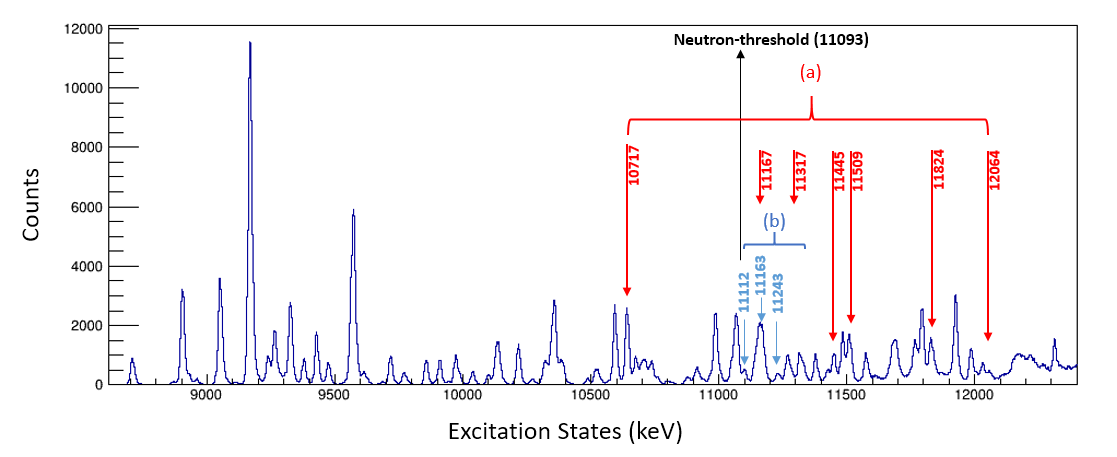
\includegraphics[scale=0.8]{graph/ch5/states2}}
    \caption{Spectrum of $^{26}$Mg in the high-lying states region (excited states above $E_x$ = 8.706 MeV) measured by this work. Energy regions above the $\alpha$ threshold probed by Talwar\citep{Rashi2016} and Massimi\citep{MASSIMI2017} are quoted by red (a) and blue (b) bracket, respectively. The red arrows and values indicate the states that were also observed by Talwar and the blues ones indicate the work by Massimi in units of keV.}
    \label{fig:states2}
    \end{figure}
\end{landscape}

\begin{landscape}
\begin{center}
%\setlength{\LTleft}{0pt} \setlength{\LTright}{0pt}
%\setlength{\tabcolsep}{7mm}
    \begin{longtable}{cc cc cc cc cc}
    %\setlength{\LTleft}{0pt} \setlength{\LTright}{0pt}
    \caption{COMPARISONS WITH STATES of $^{26}$MG POPULATED BY THE (D,P) and (N,$\gamma$) N-TOF REACTIONS \label{tb:dp}\/}\\
    \toprule
    \hline
    \multicolumn{2}{c}{This Work} & \multicolumn{2}{c}{Cujec $et\ al.$\citep{Cujec1964}}  & \multicolumn{2}{c}{Hinds $et\ al.$\citep{Hinds1965}\citep{Hinds1961}}&\multicolumn{2}{c}{Arciszewski $et\ al.$\citep{Arciszewski1984}}& \multicolumn{2}{c}{Massimi $et\ al.$\citep{Massimi}\citep{MASSIMI2017}}       \\
    \multicolumn{2}{c}{($d,p$)}   & \multicolumn{2}{c}{($d,p$)}          & \multicolumn{2}{c}{$(d,p)$}        &  \multicolumn{2}{c}{$(d,p)$}            & \multicolumn{2}{c}{$(n,\gamma)$n-ToF}         \\
      $E_x$(MeV)&    $l_n$        &  $E_x$(MeV)   & $l_n$                & $E_x$(MeV)     &     $l_n$         &  $E_x$(MeV)     &     $l_n$             & $E_x$(MeV)          &    $l_n$              \\
    \midrule
    \endfirsthead % Everything above goes at the top of the 1st page only
% As with the first header, we don't want obscene amounts of space for
% subsequent headings either, and eliminate an em of whitespace.
  \caption[]{{\em Continued}}\\
    \midrule
    \hline
    \multicolumn{2}{c}{This Work} & \multicolumn{2}{c}{Cujec $et\ al.$\citep{Cujec1964}}  & \multicolumn{2}{c}{Hinds $et\ al.$\citep{Hinds1965}\citep{Hinds1961}}&\multicolumn{2}{c}{Arciszewski $et\ al.$\citep{Arciszewski1984}}& \multicolumn{2}{c}{Massimi $et\ al.$\citep{Massimi}\citep{MASSIMI2017}}       \\
    \multicolumn{2}{c}{($d,p$)}   & \multicolumn{2}{c}{($d,p$)}          & \multicolumn{2}{c}{$(d,p)$}        &  \multicolumn{2}{c}{$(d,p)$}            & \multicolumn{2}{c}{$(n,\gamma)$n-ToF}         \\
      $E_x$(MeV)&    $l_n$        &  $E_x$(MeV)   & $l_n$                & $E_x$(MeV)     &     $l_n$         &  $E_x$(MeV)     &     $l_n$             & $E_x$(MeV)          &     $l_n$             \\

    \midrule
    \endhead
    \endfoot % The above section goes at the bottom of continuation pages
  \bottomrule

\endlastfoot


	&		&	0	&		&	0	&	2	&	0	&	2	&		&		\\
1.810(11) 	&		&	1.81	&		&	1.805	&	0+2	&	1.809	&	0,2	&		&		\\
2.940(11) 	&		&	2.94	&		&	2.941	&	0	&	2.938	&	0	&		&		\\
3.583(11) 	&		&	3.58	&	2	&	3.584	&	2	&	3.588	&	2	&		&		\\
3.940(12) 	&		&	3.94	&		&	3.943	&	0	&	3.941	&	0,2	&		&		\\
	&		&	4.32	&		&	4.319	&		&		&		&		&		\\
4.330(11) 	&		&	4.33	&		&	4.331	&		&		&		&		&		\\
4.340(11) 	&		&	4.35	&		&	4.350	&		&		&		&		&		\\
4.831(11) 	&		&	4.83	&	(1,0)	&	4.830	&	0	&	4.834	&	0,2	&		&		\\
4.904(12) 	&		&	4.90	&	2	&	4.896	&	2	&	4.900	&	2	&		&		\\
	&		&	4.97	&		&	4.970	&	2	&		&	2	&		&		\\
5.291(12) 	&		&	5.29	&		&	5.287	&	2	&	5.291	&	2	&		&		\\
5.464(12) 	&		&	5.47	&		&	5.472	&	2	&	5.474	&	2	&		&		\\
5.693(11) 	&		&	5.69	&		&	5.686	&		&		&	0,2	&		&		\\
5.709(12) 	&		&	5.71	&		&	5.710	&		&	5.716	&	0,2	&		&		\\
6.121(12) 	&		&	6.12	&	(0+2)	&	6.120	&	0	&	6.125	&	1	&		&		\\
6.253(12) 	&		&	6.25	&		&	6.253	&		&		&	1,3	&		&		\\
6.617(11) 	&		&	6.62	&	(2+0)	&	6.616	&		&		&	1,3	&		&		\\
6.732(12) 	&		&	6.74	&	(2+0)	&	6.737	&		&	6.744	&	1,3	&		&		\\
6.875(12) 	&		&	6.87	&		&	6.870	&		&	6.878	&	2	&		&		\\
6.967(11) 	&		&	6.97	&		&	6.967	&		&		&	2	&		&		\\
7.058(11) 	&		&	7.06	&		&	7.053	&		&		&	0,2	&		&		\\
7.096(11) 	&		&	7.10	&		&	7.096	&		&		&	3	&		&		\\
7.198(12) 	&		&	7.24	&		&	7.237	&		&	7.262 + 7.282	&		&		&		\\
7.251(10) 	&		&	7.25	&		&	7.251	&		&		&		&		&		\\
7.269(11) 	&		&	7.27	&		&	7.273	&		&		&		&		&		\\
7.347(12) 	&		&	7.34	&		&	7.338	&		&	7.347	&		&		&		\\
	&		&	7.35	&		&	   	&		&		&		&		&		\\
	&		&	7.38	&		&	7.383	&		&		&		&		&		\\
	&		&	7.41	&		&	7.414	&		&		&		&		&		\\
  7.540 (11)  	&		&	7.53	&		&	7.528	&		&	7.543	&		&		&		\\
	&		&	7.67	&		&	7.668	&		&		&		&		&		\\
  7.677 (11)  	&		&	7.68	&		&	   	&		&		&		&		&		\\
  7.712 (12)  	&		&	7.71	&		&	7.714	&		&	7.723	&		&		&		\\
  7.733 (11)  	&		&		&		&		&		&		&		&		&		\\
	&		&	7.76	&		&	7.761	&		&	7.771	&		&		&		\\
  7.809 (11)  	&		&	7.81	&	1	&	7.808	&		&	7.815	&		&		&		\\
	&		&	7.83	&		&	7.842	&		&		&		&		&		\\
  7.942 (10)  	&		&	7.94	&		&	7.945	&		&	7.950	&		&		&		\\
  7.996 (11)  	&		&	8.02	&		&	8.020	&		&		&		&		&		\\
  8.042 (11)  	&		&	8.04	&		&	8.040	&		&		&		&		&		\\
  8.179 (12)  	&		&	8.17	&		&	8.175	&		&		&		&		&		\\
	&		&	(8.19)	&		&	  	&		&		&		&		&		\\
  8.243 (12)  	&		&	8.24	&	0	&	8.243	&		&		&		&		&		\\
  8.393 (11)  	&		&	8.39	&		&	8.388	&		&		&		&		&		\\
  8.454 (10)  	&		&	8.45	&		&	8.451	&		&		&		&		&		\\
  8.497 (11)  	&		&	8.49	&		&	8.494	&		&		&		&		&		\\
  8.527 (11)  	&		&	8.52	&		&	8.524	&		&		&		&		&		\\
	&		&	8.57	&		&	8.565	&		&		&		&		&		\\
  8.621 (11)  	&		&	8.62	&		&	8.617	&		&		&		&		&		\\
	&		&	8.66	&		&		&		&		&		&		&		\\
  8.706 (11)  	&		&	8.69	&		&		&		&		&		&		&		\\
   8.865(11)  	&		&	8.85	&		&		&		&		&		&		&		\\
  8.904 (10)  	&		&	8.89	&		&		&		&		&		&		&		\\
8.931(11)	&		&	8.92	&		&		&		&		&		&		&		\\
  8.960 (11)  	&		&	8.95	&		&		&		&		&		&		&		\\
	&		&	9.03	&	0	&		&		&		&		&		&		\\
   9.052(11)  	&		&	9.05	&		&		&		&		&		&		&		\\
	&		&	9.10	&		&		&		&		&		&		&		\\
  9.167 (11)  	&		&	9.16	&		&		&		&		&		&		&		\\
  9.238 (12)  	&		&	9.22	&		&		&		&		&		&		&		\\
  9.263 (11)  	&		&	9.25	&		&		&		&		&		&		&		\\
   9.322(11)  	&		&	9.30	&		&		&		&		&		&		&		\\
  9.382 (11)  	&		&	9.37	&	0	&		&		&		&		&		&		\\
  9.430 (11)  	&		&	9.42	&	0	&		&		&		&		&		&		\\
  9.476 (11)  	&		&	9.46	&		&		&		&		&		&		&		\\
	&		&	9.53	&		&		&		&		&		&		&		\\
   9.578(11)  	&		&	9.56	&		&		&		&		&		&		&		\\
   9.613(11)  	&		&	9.62	&		&		&		&		&		&		&		\\
  9.683 (10)  	&		&	9.67	&		&		&		&		&		&		&		\\
  9.716 (11)  	&		&	9.71	&		&		&		&		&		&		&		\\
  9.770 (11)  	&		&	9.76	&		&		&		&		&		&		&		\\
	&		&	9.81	&		&		&		&		&		&		&		\\
  9.856 (11)  	&		&	9.84	&		&		&		&		&		&		&		\\
  9.991 (11)  	&		&	9.90	&		&		&		&		&		&		&		\\
  9.985 (11)  	&		&	9.93	&		&		&		&		&		&		&		\\
	&		&	9.97	&		&		&		&		&		&		&		\\
  10.040(10)  	&		&	10.03	&		&		&		&		&		&		&		\\
  10.100(10)  	&		&	10.09	&		&		&		&		&		&		&		\\
  10.137(11)  	&		&	10.12	&		&		&		&		&		&		&		\\
	&		&	10.21	&		&		&		&		&		&		&		\\
  10.269(11)  	&		&	10.27	&		&		&		&		&		&		&		\\
  10.320(11)  	&		&	10.32	&		&		&		&		&		&		&		\\
  10.355(12)  	&		&	10.36	&		&		&		&		&		&		&		\\
  10.385(12)  	&		&	10.40	&		&		&		&		&		&		&		\\
	&		&	10.42	&		&		&		&		&		&		&		\\
  10.487(12)  	&		&	10.48	&		&		&		&		&		&		&		\\
  10.522(11)  	&		&	10.52	&		&		&		&		&		&		&		\\
10.568(11)	&		&		&		&		&		&		&		&		&		\\
  10.595(11)  	&		&	10.59	&		&		&		&		&		&		&		\\
     10.641(11) 	&		&	10.64	&		&		&		&		&		&		&		\\
     10.676(11) 	&		&		&		&		&		&		&		&		&		\\
     10.708(10) 	&	1	&	10.70	&		&		&		&		&		&		&		\\
     10.735(11) 	&	2	&		&		&		&		&		&		&		&		\\
     10.808(10) 	&	2	&		&		&		&		&		&		&		&		\\
     10.875(11) 	&	3	&		&		&		&		&		&		&		&		\\
     10.915(10) 	&	2	&	10.91	&		&		&		&		&		&		&		\\
   10.988(11)   	&	3	&	10.98	&		&		&		&		&		&		&		\\
	&		&	11.00	&		&		&		&		&		&		&		\\
    11.069(10)  	&	2	&	11.07	&		&		&		&		&		&		&		\\
     11.112(11) 	&	3	&	11.12	&		&		&		&		&		&	11.112	&	0	\\
	&		&		&		&		&		&		&		&	11.154	&	1	\\
	&		&		&		&		&		&		&		&	11.163	&	0	\\
    11.165(10)  	&	1	&	11.16	&		&		&		&		&		&	11.169	&	(0)	\\
	&		&		&		&		&		&		&		&	11.171	&	0	\\
	&		&		&		&		&		&		&		&	11.183	&	1	\\
	&		&	11.22	&		&		&		&		&		&	11.190	&	0	\\
    11.232(10)  	&	2	&		&		&		&		&		&		&	11.243	&	(1)	\\
    11.267(10)  	&	2	&		&		&		&		&		&		&	11.274	&	0	\\
	&		&	11.28	&		&		&		&		&		&	11.280	&	(1	\\
	&		&		&		&		&		&		&		&	11.285	&	1	\\
	&		&		&		&		&		&		&		&	11.289	&	(1)	\\
	&		&		&		&		&		&		&		&	11.295	&	(1)	\\
    11.317(11)  	&	3	&	11.31	&		&		&		&		&		&	11.328	&	1	\\
	&		&	11.34	&		&		&		&		&		&	11.344	&	(1)	\\									
    11.374(12)  	&	3	&	11.38	&		&		&		&		&		&	11.362	&	(0)	\\
    11.425(12)  	&	2	&		&		&		&		&		&		&				\\
	&		&		&		&		&		&		&		&	11.393	&	(2)	\\
	&		&		&		&		&		&		&		&		&		\\
    11.447(11)  	&	3	&	11.45	&		&		&		&		&		&	11.441	&	2	\\
	&		&		&		&		&		&		&		&	11.466	&	(3)	\\
    11.482(10)  	&	1	&	11.48	&		&		&		&		&		&		&		\\
    11.509(10)  	&	3	&	11.51	&		&		&		&		&		&	11.500	&	1	\\
	&		&		&		&		&		&		&		&	11.527	&	(1)	\\
     11.573(11) 	&	3	&	11.57	&		&		&		&		&		&		&		\\
	&		&		&		&		&		&		&		&	11.592	&	(1)	\\
     11.613(11) 	&	2	&	11.60	&		&		&		&		&		&	11.613	&	(1)	\\
   11.690(10)   	&	1	&	11.69	&		&		&		&		&		&		&		\\
   11.767(11)   	&	3	&	11.76	&		&		&		&		&		&		&		\\
   11.790(11)   	&	2	&	11.79	&		&		&		&		&		&		&		\\
   11.828(10)   	&	3	&	11.83	&		&		&		&		&		&		&		\\
     11.874(11) 	&	2	&	11.90	&		&		&		&		&		&		&		\\
    11.927(11)  	&	3	&		&		&		&		&		&		&		&		\\
    11.981(11)  	&	2	&		&		&		&		&		&		&		&		\\
     12.032(11) 	&	1	&	12.00	&		&		&		&		&		&		&		\\
     12.059(12) 	&	3	&		&		&		&		&		&		&		&		\\
    12.311(11)  	&	1	&		&		&		&		&		&		&		&		\\
	&		&	12.50	&		&		&		&		&		&		&		\\
	&		&	12.57	&		&		&		&		&		&		&		\\

    \end{longtable}
\end{center}
\end{landscape}



\subsection{Comparison with the reactions $^{23}$Na($\alpha$,p$\gamma$)$^{26}$Mg and $^{12}$C($^{18}$O,$\alpha$)$^{26}$Mg}
In addition to the reactions mentioned above, more methods have been used to explore the high-spin states ($J>4$) in $^{26}$Mg, including the proton-$\gamma$-ray coincidence measurements in the $^{23}$Na($\alpha$,p$\gamma$)$^{26}$Mg (Glatz $et\ al.$\citep{Glatz1986}) and the heavy-ion reactions by $^{12}$C($^{18}$O,$\alpha$)$^{26}$Mg (Gustafson $et\ al.$ \citep{Gustafson1976}), as listed in Table~\ref{tb:other}. Though both reactions are dependable ways of investigating high-spin states, the spin-parity assignments obtained in these works showed limited agreement, possibly due to the fact that \citep{Glatz1986} used the particle-$\gamma$-ray angular correlation method while \citep{Gustafson1976} predicted them by Hauser-Feshbach (HF) calculation.

The neutron-transfer reaction performed in this work can only give the possible $l_n$ values. The $J^{\pi}$ values associated with   $l_n$s are  $J^{\pi}=2^+$ for $l_n=$0;
$J^{\pi}=1^-,3^-$ for $l_n=$1;
$J^{\pi}=0^+,2^+,4^+$ for $l_n=$2;
$J^{\pi}=1^-,3^-,5^-$ for $l_n=$3, etc., which does not provide sufficient information for high-spin(-parity) assignments except  states with $l_n=$3 , for example, $E_x=$11.537(11) MeV and 11.767(11) MeV potentially agree with \citep{Gustafson1976}'s calculation.



\begin{center}
%\setlength{\LTleft}{0pt} \setlength{\LTright}{0pt}
%\setlength{\tabcolsep}{7mm}
    \begin{longtable}{cc cc cc}
    %\setlength{\LTleft}{0pt} \setlength{\LTright}{0pt}
    \caption{COMPARISONS WITH STATES of $^{26}$MG POPULATED BY OTHER REACTIONS \label{tb:other}\/}\\
    \toprule
    \hline
     \multicolumn{2}{c}{This Work} & \multicolumn{2}{c}{Glatz $et\ al.$\citep{Glatz1986}}         &\multicolumn{2}{c}{Gustafson $et\ al.$ \citep{Gustafson1976}}  \\
     \multicolumn{2}{c}{($d,p$)}   & \multicolumn{2}{c}{ ($\alpha,p\gamma$) }                     & \multicolumn{2}{c}{($^{18}O,\alpha$)}                         \\
       $E_x$(MeV)&    $l_n$        &  $E_x$(MeV)   & $J^{\pi}$                                    & $E_x$(MeV)         &           $J^{\pi}$                      \\
    \midrule
    \endfirsthead % Everything above goes at the top of the 1st page only
% As with the first header, we don't want obscene amounts of space for
% subsequent headings either, and eliminate an em of whitespace.
  \caption[]{{\em Continued}}\\
    \midrule
    \hline
     \multicolumn{2}{c}{This Work} & \multicolumn{2}{c}{Glatz $et\ al.$\citep{Glatz1986}}         &\multicolumn{2}{c}{Gustafson $et\ al.$ \citep{Gustafson1976}}  \\
     \multicolumn{2}{c}{($d,p$)}   & \multicolumn{2}{c}{ ($\alpha,p\gamma$) }                     & \multicolumn{2}{c}{($^{18}O,\alpha$)}                         \\
       $E_x$(MeV)&    $l_n$        &  $E_x$(MeV)   & $J^{\pi}$                                    & $E_x$(MeV)         &           $J^{\pi}$                      \\

    \midrule
    \endhead
    \endfoot % The above section goes at the bottom of continuation pages
  \bottomrule

\endlastfoot

  &   & 0.000 & 0 & 0 &   \\
1.810(11)   &   & 1.809 & 2 & 1.83  & (2$^+$)                 \\
2.940(11)   &   & 2.938 & 2 & 2.96  & (2$^+$)                 \\
3.583(11)   &   & 3.588 & 0 & 3.58  &                         \\
3.940(12)   &   & 3.941 & 3 & 3.96  & (3$^+$),(4$^-$)         \\
  &   & 4.318 & 4 &   &   \\
4.330(11)   &   & 4.332 & 2 & 4.32  & (2$^+$),(3$^+$)         \\
4.340(11)   &   & 4.350 & 3 &   &                         \\
4.831(11)   &   & 4.835 & 2 & 4.82  & (2$^+$)                 \\
4.904(12)   &   & 4.901 & 4 & 4.90  & (4$^+$)                 \\
  &   & 4.972 & 0 & 5.00  &                         \\
5.291(12)   &   & 5.292 & 2 & 5.31  & (2$^+$)                 \\
5.464(12)   &   & 5.475 & 4 & 5.48  & (4$^+$)                 \\
5.693(11)   &   & 5.692 & 1 & 5.68  & (1$^-$)                 \\
5.709(12)   &   & 5.715 & 4 & 5.73  & (3$^+$)                 \\
6.121(12)   &   & 6.125 & 3 & 6.17  & (2$^+$)                 \\
6.253(12)   &   & 6.256 & 0 & 6.30  & ((1$^-$, 2$^-$))        \\
6.617(11)   &   & 6.623 & 4$^+$ & 6.60  & (2$^+$)                 \\
  &   & 6.634 & 1 &   &   \\
6.732(12)   &   & 6.745 & 2 & 6.71  & (3$^-$)                 \\
6.875(12)   &   &   &   & 6.87  & ((2$^+$, 3$^+$))        \\
6.967(11)   &   & 6.978 & 5$^+$   & 6.94  & ((2$^+$, 3$^+$))        \\
7.058(11)   &   &   &   & 7.08  & (2$^+$)                 \\
7.096(11)   &   &   &   &   &   \\
7.198(12)   &   &   &   &   &   \\
7.251(10)   &   & 7.242 & 3 &   &   \\
7.269(11)   &   & 7.283 & 4$^-$ &   &   \\
7.347(12)   &   &   &   & 7.34  & ((2$^+$, 3$^+$))          \\
  &   & 7.395 & 5$^+$ & 7.42  & ((2$^+$, 3$^+$))          \\
  7.540 (11)    &   &   &   & 7.54  & ((4$^+$, 5$^+$))          \\
  7.677 (11)    &   & 7.677 & 3$^-$,4$^-$,5$^-$ & 7.64  & ((2$^+$, 3$^+$, 4$^-$))   \\
  7.712 (12)    &   &   &   & 7.72  &                           \\
  7.733 (11)    &   & 7.773 & 4 &   & ((2$^+$, 3$^+$))          \\
  7.809 (11)    &   &   &   &   &                           \\
  7.942 (10)    &   & 7.953 & 5$^-$ & 7.96  & (4$^+$)                   \\
  7.996 (11)    &   &   &   &   &                           \\
  8.042 (11)    &   &   &   & 8.07  & (4$^+$)                   \\
  8.179 (12)    &   & 8.202 & 6$^+$ & 8.16  & (3$^-$)                   \\
  8.243 (12)    &   &   &   &   &                           \\
  8.393 (11)    &   &   &   & 8.38  & (6$^+$)                   \\
  8.454 (10)    &   &   &   &   &                           \\
  8.497 (11)    &   & 8.472 & 6$^+$ & 8.50  & (6$^+$)                   \\
  8.527 (11)    &   &   &   &   &                           \\
  8.621 (11)    &   & 8.624 & 3,4,5 &   &                           \\
  8.706 (11)    &   & 8.670 & 3,5 & 8.70  & (5$^-$)                   \\
   8.865(11)    &   &   &   & 8.84  & (4$^+$)                   \\
  8.904 (10)    &   & 9.065 & 5 & 8.91  & (6$^+$)                   \\
8.931(11) &   &   &   &   &                           \\
  8.960 (11)    &   &   &   & 9.85  & ((2$^+$, 3$^+$))          \\
   9.052(11)    &   &   &   & 9.05  & ((4$^-$))                 \\
  9.167 (11)    &   & 9.112 & 6$^+$ & 9.13  & ((5$^-$,6$^-$))           \\
  9.238 (12)    &   & 9.169 & 6$^-$ & 9.22  & ((2$^+$,3$^+$))           \\
  9.263 (11)    &   &   &   &   &                           \\
   9.322(11)    &   &   &   & 9.30  & ((5$^-$, 6$^-$))          \\
  9.382 (11)    &   & 9.383 & 6$^+$ &   &   \\
  9.430 (11)    &   &   &   &   &   \\
  9.476 (11)    &   &   &   &   &   \\
  &   & 9.542 & 5 & 9.53  & ((5$^-$, 6$^-$))        \\
   9.578(11)    &   &   &   & 9.57  & (7$^-$)                 \\
   9.613(11)    &   &   &   &   &                         \\
  9.683 (10)    &   &   &   &   &                         \\
  9.716 (11)    &   &   &   &   &                         \\
  9.770 (11)    &   &   &   &   &                         \\
  9.856 (11)    &   & 9.829 & 7$^+$ & 9.84  & ((5$^-$, 7$^+$))        \\
  9.991 (11)    &   &   &             & 9.91  & ((2$^+$, 3$^+$))        \\
  9.985 (11)    &   & 9.989 & 6$^+ $      & 9.95  & (4$^-$)                 \\
  10.040(10)    &   &   &   & 10.02 & (3$^-$)                 \\
  10.100(10)    &   &   &   & 10.06 & ((3$^-$, 4$^-$))        \\
  10.137(11)    &   &   &   &   &                         \\
  &   &   &   & 10.16 & ((5$^-$, 7$^+$))        \\
  10.269(11)    &   &   &   &   &                         \\
  10.320(11)    &   &   &   &   &                         \\
  10.355(12)    &   &   &   &   &                         \\
  10.385(12)    &   &   &   &   &                         \\
  &   &   &   & 10.42 & ((3$^-$,5$^+$))         \\
  10.487(12)    &   &   &   & 10.48 & (6$^+$)                 \\
  10.522(11)    &   &   &   & 10.52 & (2$^+$)                 \\
10.568(11)  &   &   &   &   &                         \\
  10.595(11)    &   &   &   &   &                         \\
     10.641(11)   &   &   &   &   &                         \\
     10.676(11)   &   &   &   & 10.66 & ((4$^+$, 5$^+$))        \\
     10.708(10)   & 1 &   &   &   &                         \\
     10.735(11)   & 2 &   &   & 10.74 & (7$^-$)                 \\
     10.808(10)   & 2 &   &   &   &   \\
     10.875(11)   & 3 &   &   &   &   \\
     10.915(10)   & 2 &   &   &   &   \\
   10.988(11)     & 3 &   &   & 10.96 & (7$^-$)                   \\
    11.069(10)    & 2 &   &   & 11.08 & ((4$^+$, 6$^-$))          \\
     11.112(11)   & 3 &   &   &   &                           \\
    11.165(10)    & 1 &   &   & 11.16 & ((6$^+$, 8$^-$))          \\
    11.232(10)    & 2 &   &   &   &                           \\
    11.267(10)    & 2 &   &   &   &                           \\
    11.317(11)    & 3 &   &   & 11.31 & (7$^-$)                   \\
    11.374(12)    & 3 & 11.392  & 7 &   &                           \\
    11.425(12)    & 2 &   &   & 11.42 & ((5$^-$, 7$^+$))          \\
    11.447(11)    & 3 &   &   & 11.45  & ((5$^-$, 7$^+$))            \\
    11.482(10)    & 1 &   &   &   &                           \\
    11.509(10)    & 3 &   &   & 11.51 & ((4$^+$, 6$^-$))          \\
     11.573(11)   & 3 & 11.570  & 7 & 11.56 & ((5$^-$, 6$^-$))          \\
     11.613(11)   & 2 &   &   &   &                           \\
  &   &   &   & 11.64 & (8$^+$)                   \\
   11.690(10)     & 1 &   &   &   &                           \\
   11.767(11)     & 3 &   &   & 11.77 & ((5$^-$, 7$^+$))          \\
   11.790(11)     & 2 &   &   &   &                           \\
  &   &   &   &   &                           \\
   11.828(10)     & 3 &   &   & 11.83 & (6$^+$)                   \\
     11.874(11)   & 2 &   &   &   &                           \\
    11.927(11)    & 3 &   &   & 11.94 & ((6$^+$, 8$^-$))          \\
    11.981(11)    & 2 &   &   &   &                           \\
     12.032(11)   & 1 &   &   & 12.03 & ((7$^-$, 9$^+$))          \\
     12.059(12)   & 3 &   &   &   &                           \\
  &   &   &   & 12.10 & ((6$^+$, 8$^-$))          \\
  &   &   &   & 12.14 & ((6$^+$, 8$^-$))          \\
  &   &   &   & 12.20 & ((6$^+$, 9$^+$))          \\
  &   &   &   & 12.28 & ((4$^+$, 5$^+$, 6$^-$))   \\
    12.311(11)    & 1 &   &   & 12.34 & ((5$^-$, 7$^+$))          \\
  &   &   &   & 12.40 & ((6$^+$, 8$^-$))          \\
  &   & 12.479  & 8$^-$,7$^+$ & 12.45 & (6$^+$)                   \\
  &   &   &   & 12.53 & (8$^+$)                   \\
  &   &   &   & 12.63 & ((6$^+$, 8$^+$))          \\
  &   &   &   & 12.88 & ((6$^+$, 8$^-$))          \\
  &   &   &   & 12.95 & ((7$^-$, 9$^+$))          \\
  &   &   &   & 13.00 & ((6$^+$, 9$^+$))          \\
  &   &   &   & 13.06 & ((6$^+$, 9$^+$))          \\
  &   &   &   & 13.12 & (7$^-$)                   \\
  &   &   &   & 13.19 & (8$^+$)                   \\
  &   &   &   & 13.25 & ((7$^-$, 9$^+$))          \\
  &   &   &   & 13.35 & ((6$^+$, 7$^-$, 9$^+$))   \\
  &   &   &   & 13.39 & (9$^+$)                   \\
  &   &   &   & 13.46 & ((6$^+$, 8$^-$))          \\
  &   &   &   & 13.52 & (9$^+$)                   \\
  &   &   &   & 13.59 & (8$^+$)                   \\
  &   &   &   & 13.64 & (9$^-$)                   \\
  &   &   &   & 13.69 & ((6$^+$, 8$^-$))          \\
  &   &   &   & 13.75 & ((6$^+$, 8$^-$))          \\
  &   &   &   & 13.85 & (8$^+$)                   \\
  &   &   &   & 13.90 & ((7$^-$, 8$^+$))          \\
  &   &   &   & 13.955  & (7$^-$)                   \\
  &   &   &   & 14.08 &   (9$^-$)                 \\
  &   &   &   & 14.14 &   ((9$^-$, 10$^+$))       \\
  &   &   &   & 14.21 &   (9$^-$)                 \\
  &   &   &   & 14.30 &   (8$^+$)                 \\
  &   &   &   & 14.38 &   (7$^-$)                 \\
  &   &   &   & 14.50 &   (8$^+$)                 \\
  &   &   &   & 14.56 &   ((7$^-$, 9$^+$))        \\
  &   &   &   & 14.62 &   (6$^+$)                 \\
  &   &   &   & 14.66 &   ((6$^+$, 8$^-$))        \\
  &   &   &   & 14.70 &   ((7$^-$, 8$^+$))        \\
  &   &   &   & 14.75 &   ((8$^+$,9$^-$))         \\
  &   &   &   & 14.86 &   (8$^+$)                 \\
  &   &   &   & 14.92 &   (8$^+$)                 \\
  &   &   &   & 14.96 &   (8$^+$)                 \\
  &   &   &   & 15.00 &   (8$^+$)                 \\
  &   &   &   & 15.14 &   (8$^+$)                 \\
  &   &   &   & 15.21 &   ((8$^+$, 9$^-$))        \\
  &   &   &   & 15.35 &   (8$^+$)                 \\
  &   &   &   & 15.4  &   (9$^-$)                 \\
  &   &   &   & 15.46 &   ((9$^-$, 10$^+$))       \\
  &   &   &   & 15.56 &   (8$^+$)                 \\
  &   &   &   & 15.70 &   ((9$^-$, 10$^+$))       \\
  &   &   &   & 15.77 &   (8$^+$)                 \\
  &   &   &   & 15.84 &   (9$^-$)                 \\
  &   &   &   & 15.91 &   ((8$^+$, 9$^-$))        \\
  &   &   &   & 15.98 &   (7$^+$)                 \\
  &   &   &   & 16.04 &   (7$^-$)                 \\
  &   &   &   & 16.10 &   (7$^-$)                 \\
  &   &   &   & 16.20 &   (8$^+$)                 \\
  &   &   &   & 16.26 &   (9$^-$)                 \\
  &   &   &   & 16.35 &   ((8$^+$, 9$^-$))        \\

    \end{longtable}
\end{center}




\section{Angular Distribution Analysis}
As mentioned in Chapter 4, the Grand Raiden spectrometer was operated in 3 angle modes including the 0$^{\circ}$ mode, so that measurements can be taken in the angular range from 0.5$^{\circ}$ to about 45$^{\circ}$ of the high-lying states (the 3rd setting B3). The measurements of the angular distributions will help to determine the orbital momentum of the transferred neutron by comparing the experimental data with   Distorted Wave Born Approximation (DWBA) calculations. In this work, the DWUCK4 code~\citep{DWUCK4} was used for the DWBA calculations since it based on the zero range correction and provided the well-studied fitting parameters for the (d,p) reaction ~\citep{DWUCK4}.

\begin{center}
  \begin{longtable}{lcccccccccccc}
    \caption{OPTICAL POTENTIAL  PARAMETERS  USED IN THE DWBA ANALYSIS OF $^{25}$Mg(d,p)$^{26}$Mg ~\citep{HATANAKA1984530} \label{tbl:opticalpotential}\/}\\
        \toprule
        \toprule
         Target  &  & $V_0$   & $r_0$  & $a_0$   &  $W_v$  & $W_D$  & $r_W$ & $a_W$  & $V_{LS}$  & $r_{LS}$ & $a_{LS}$ & $r_c$  \\
         nucleus &  &  MeV  &  fm  & fm    &   MeV & MeV  & fm  & fm   &  MeV    &   fm   &   fm   & fm \\
        \midrule
\endfirsthead

\endhead % Everything above here (and below the \endfirsthead) goes at the top
         % of continuation pages.  The [] argument prevents a duplicate
         % entry from appearing in the table of contents.
% The following 3 lines are provided as an example only -- per ND
% guidelines, the footer at the bottom of a page for a longtable
% should not have a bottom line.  Only the absolute bottom of the
% table should have a final \bottomline

%  \midline
%  \multicolumn{6}{|r|}{\textit{continued}\ldots} \\
%  \bottomrule
\endfoot % The above section goes at the bottom of continuation pages
  \bottomrule
\endlastfoot % The very last bottom of the table
   $^{25}$Mg    &d & 74.05   &  1.17  &   0.804 &   3.81  &  9.90  & 1.325 &  0.731 &   3.51  &   1.07 &  0.66  & 1.3  \\
                &p & 37.57   &  1.144 &   0.69  &   9.88  &  0.0   & 1.32  &  0.657 &   5.6   &   1.01 &  0.6   & 1.25 \\
  \end{longtable}
\end{center}

The optical potential parameters used in the DWBA analysis of $^{25}$Mg(d,p)$^{26}$Mg is listed in Table~\ref{tbl:opticalpotential}. This set of parameters is first applied to the low energy $^{13}$C data measured in this experiment and compared with Hatanaka's measurement~\citep{HATANAKA1984530} in order to verify the reproducibility. As shown in Fig.~\ref{fig:13C}, the DWBA calculation in this experiment is consistent with Hatanaka's work, which proves that the optical potential parameters provided by Hatanaka should also work in our calculations.



\begin{landscape}
\begin{figure}[tpb]
  \begin{center}
    \centerline{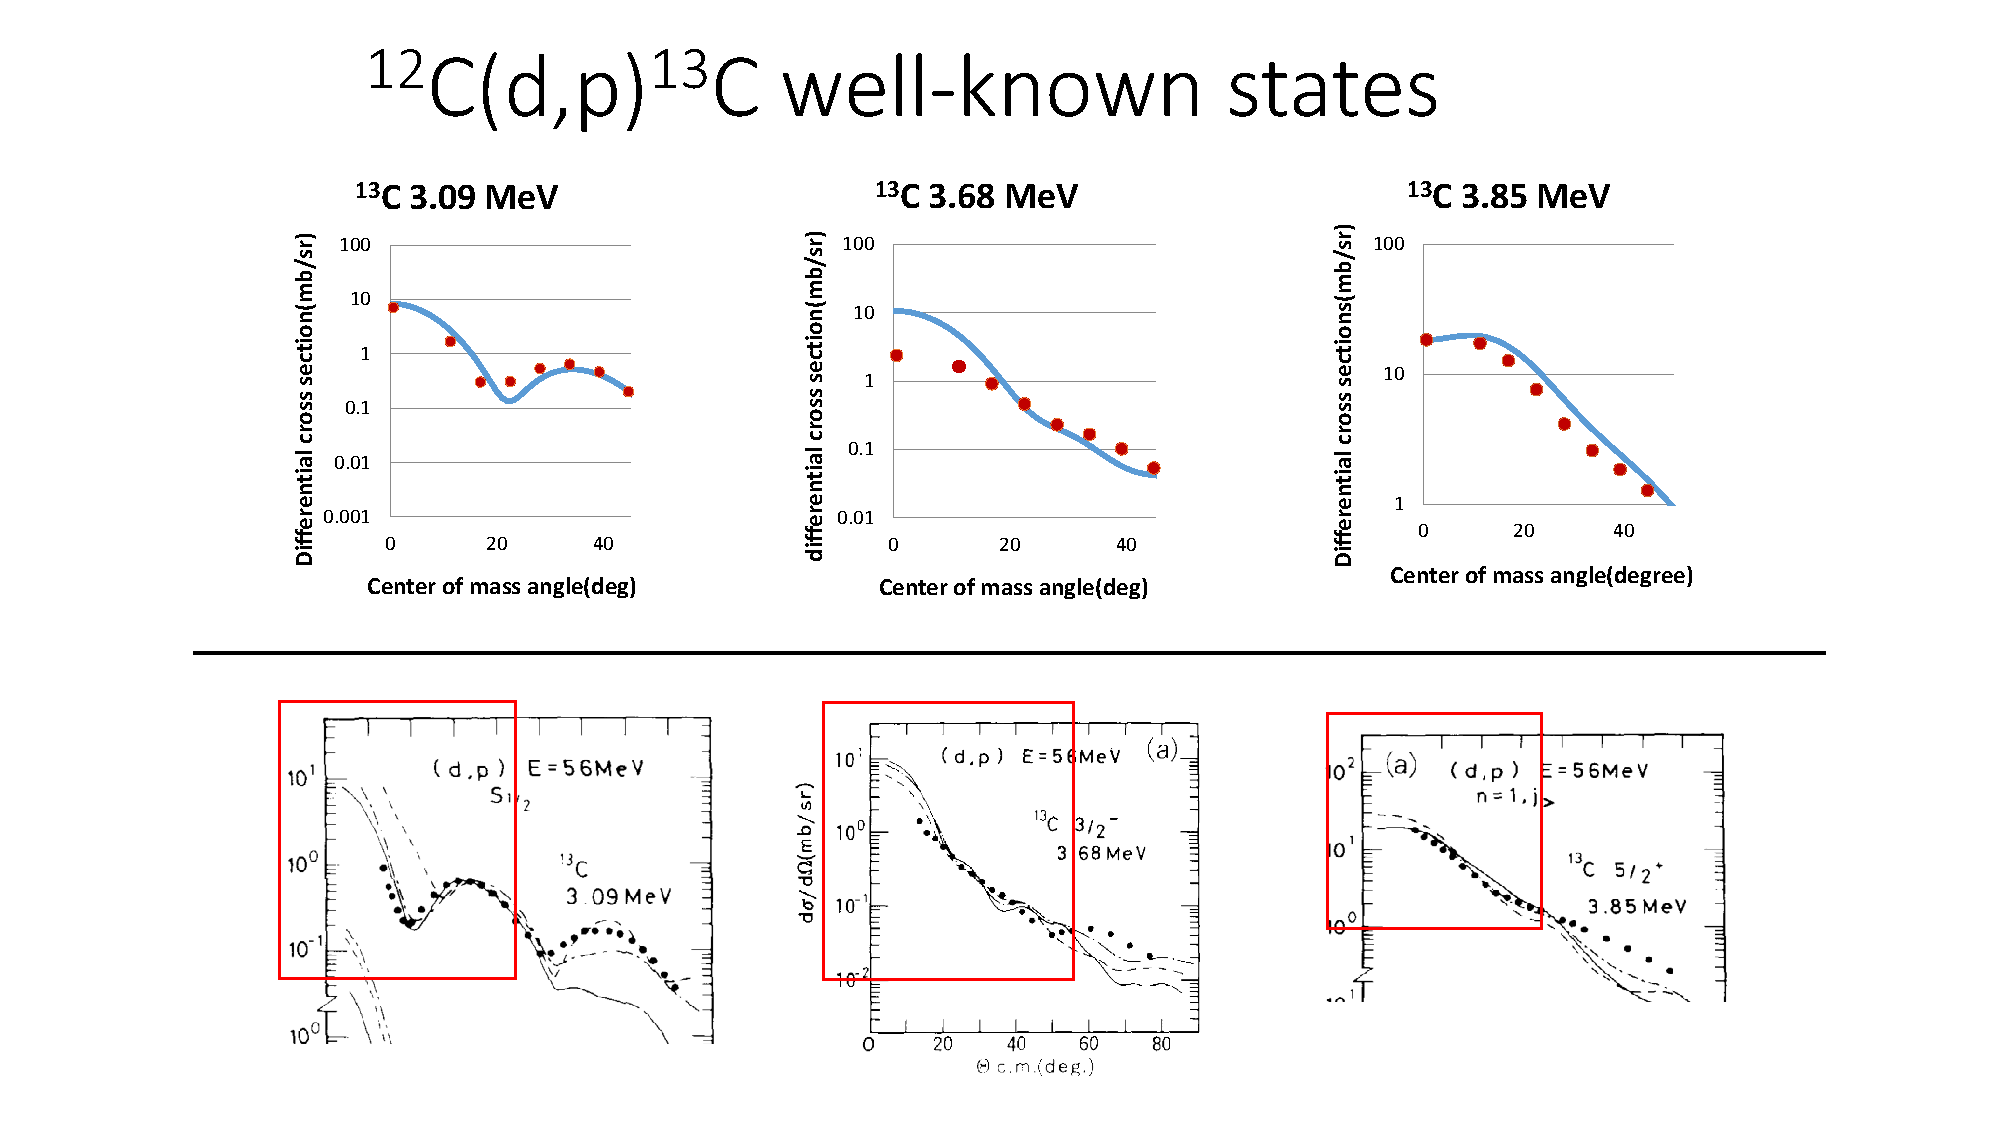
\includegraphics[scale=0.6]{graph/ch5/13C}}
    \caption{Top panel: Angular distributions using DWUCK4 for excited states obtained from the work ( The $^{12}$C(d,p)$^{13}C$ reaction at 56 MeV). Bottom panel: The comparison with results from \citep{HATANAKA1984530} using the same set of optical potential parameters.  }
    \label{fig:13C}
  \end{center}
\end{figure}
\end{landscape}

\begin{landscape}
    \begin{figure}[tpb]
    \centerline{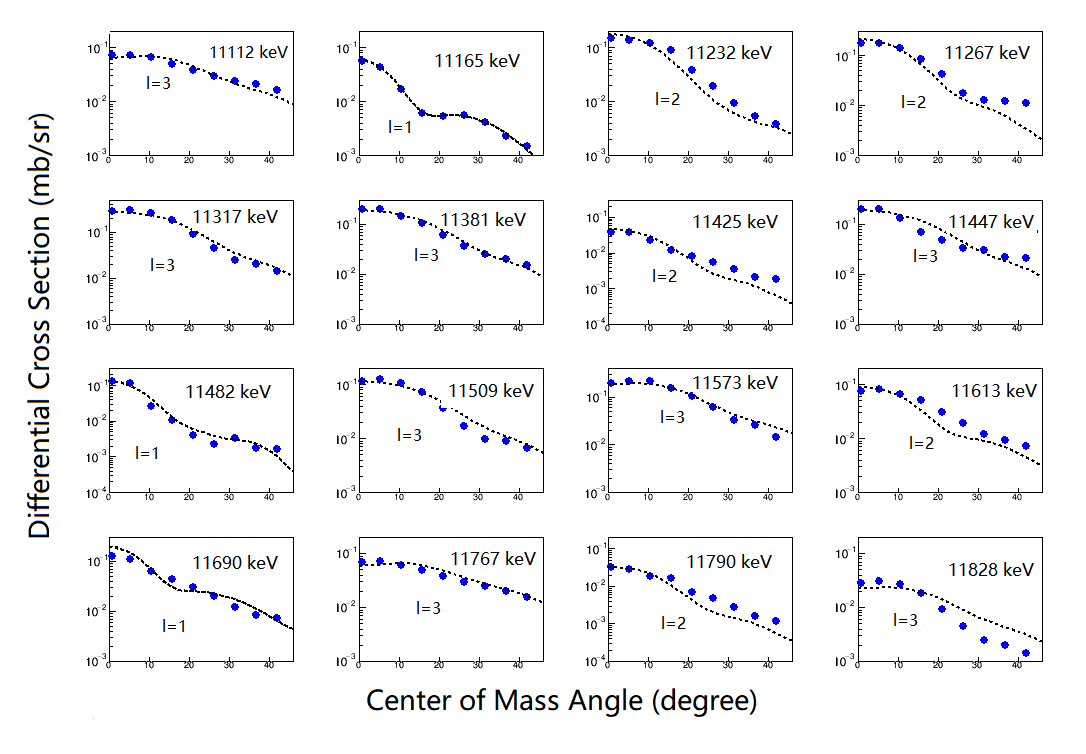
\includegraphics[scale=0.7]{graph/ch5/dwba}}
    \caption{Angular distributions using DWUCK4 for excited states above the neutron threshold obtained from $^{25}$Mg(d,p)$^{26}$Mg reaction at 56 MeV, where $l_n$ is the orbital momentum of the transferred neutron. }
    \label{fig:26Mg}
    \end{figure}
\end{landscape}


The DWBA calculations are then  performed for the high-lying states from 8.706 MeV to  12.311 MeV for the measured angular distributions. The  angular distributions and the DWBA calculations are shown in Fig.~\ref{fig:26Mg}. The possible orbital momenta of the transferred neutron of these states are listed in Tables in the last section.

In the low energy region , there is no measurement for the spin orbital assignment. However, Cujec and Hinds  performed the DWBA calculation  and assignment the J$^{\pi}$ value for some states as listed in Table~\ref{tb:dp}.
Hinds showed some angular distributions and the large cross sections at backward angles are clear indications for   contributions from Compound Nucleus reactions. Cujac only measured two angles but the list of states extends into the $\alpha$-unbound range but has large energy errors. DWBA  calculations are not really appropriate at low energies, nevertheless Hinds fits some
$l_n$-values to the forward angles. In general, these low-lying states are strongly populated in this work, the same as those populated in works of Hinds and Cujec  by either (d,p) reaction and (t,p) reaction.
In the astrophysically important excitation energy region the  level density is high in $^{26}$Mg  above the alpha threshold. For the (d,p) reaction the relative neutron  spectroscopic factors $S_n(rel)$ are extracted from transfer reactions by a comparison of experimental cross sections and the result of DWBA calculations by
\begin{equation}
    \label{eq:S_n}
    \begin{aligned}
\frac{d\sigma_{exp}}{d\Omega} = S_n(rel) N \sigma_{DWBA}
        \end{aligned}
\end{equation}
where N refers to the normalization constant i.e. N = 1.55 for (d,p) reactions~\citep{DWUCK4}.

The neutron widths $\Gamma_{n}$ of unbound states are correlated to the spectroscopic factors $S_n(rel)$ by~\citep{SCHIFFER1963246}:
\begin{equation}
    \label{eq:width_n}
    \begin{aligned}
\Gamma_{n} &=  S_n(rel)\times \Gamma_{sp}
        \end{aligned}
\end{equation}
where $\Gamma_{sp}$ is the calculated neutron single-particle width using the optical potential parameters listed in Table~\ref{tbl:opticalpotential} by DWUCK4.
The resulting resonance parameters for the resonances contributed to the region of interests have  been listed in Table~\ref{tb:reaction_parameters} along with the corresponding reaction rates in this (d,p) measurements.

\begin{landscape}
\setlength{\capwidth}{0.7\textwidth}

    \begin{table}[tpb]
        \begin{centering}
        \caption{ The $^{26}$Mg resonance parameters and the corresponding excitation energies above the neutron-threshold observed in the present work. }
        \label{tb:reaction_parameters}
    \begin{tabular}{c c c c c c c c }
    \toprule
    \toprule
    E$_x$   &       E$_R^{c.m.}$&   l$_n$    &   $\Gamma_{sp}$   &   (2J+1)$S_n$ &  (2J+1)$\Gamma_n$    &  $\Gamma_\gamma$ & $\omega\gamma_{(\alpha,\gamma)}$    \\
    keV     &       keV         &   $\hbar$  &   eV              &               &  eV                  &   eV        &          eV       \\
 \hline


        \hline
     \end{tabular}
      \end{centering}
    \end{table}

\end{landscape}

%\section{Discussion}


% % uncomment the following lines,
% if using chapter-wise bibliography
%
% \bibliographystyle{ndnatbib}
% \bibliography{example}


